\documentclass[a4paper,11pt]{article}

\usepackage[utf8]{inputenc}
\usepackage[swedish]{babel}
\usepackage[top=1in,bottom=1in,left=1in,right=1in,headsep=.5in]{geometry}
\usepackage[table]{xcolor}
\usepackage{hyperref}
\usepackage{graphicx}
\usepackage{pdfpages}
\usepackage{siunitx}
\usepackage{bytefield}
\usepackage{dirtree}
\usepackage{listings}

\usepackage{tikz}
\usetikzlibrary{shapes.geometric, shapes.misc, arrows, calc}

\usepackage{array}
\newcolumntype{L}[1]{>{\raggedright\let\newline\\\arraybackslash\hspace{0pt}}m{#1}}
\newcolumntype{C}[1]{>{\centering\let\newline\\\arraybackslash\hspace{0pt}}m{#1}}
\newcolumntype{R}[1]{>{\raggedleft\let\newline\\\arraybackslash\hspace{0pt}}m{#1}}

\usepackage[yyyymmdd,hhmmss]{datetime}
\renewcommand{\dateseparator}{-}

\usepackage{mathptmx}    %Times Roman font
\usepackage{helvet}    %Helvetica, served as a model for arial
\usepackage{anyfontsize}

\usepackage[tocgraduated]{tocstyle}
\usetocstyle{allwithdot}

\usepackage[titletoc,title]{appendix}

\usepackage[backend=bibtex,style=authoryear,maxcitenames=2,maxbibnames=9]{biblatex} %Harvard-style citations
\setlength{\bibitemsep}{\baselineskip}	%vertical space between bibliography items

\usepackage{fancyhdr}
\fancypagestyle{intro}{
    \fancyhf{}
    \fancyhead[C]{\LIPSprojekttitel}
    \fancyhead[R]{\today} 
    \fancyfoot[L]{\LIPSkursnamn \\ \LIPSdokumenttyp}
    \fancyfoot[C]{\phantom{text}\roman{page}}
    \fancyfoot[R]{\LIPSprojektgrupp \\ \LIPSgruppepost} 
    \renewcommand{\headrulewidth}{0.4pt}
    \renewcommand{\footrulewidth}{0.4pt}}
\fancypagestyle{content}{
    \fancyhf{}
    \fancyhead[C]{\LIPSprojekttitel}
    \fancyhead[R]{\today} 
    \fancyfoot[L]{\LIPSkursnamn \\ \LIPSdokumenttyp}
    \fancyfoot[C]{\phantom{text}\thepage}
    \fancyfoot[R]{\LIPSprojektgrupp \\ \LIPSgruppepost} 
    \renewcommand{\headrulewidth}{0.4pt}
    \renewcommand{\footrulewidth}{0.4pt}}

\usepackage{titlesec}
\titleformat{\section}
    {\normalfont\sffamily\Large\bfseries}
    {\thesection}{1em}{}
\titleformat{\subsection}
    {\normalfont\sffamily\large\bfseries}
    {\thesubsection}{1em}{}
\titleformat{\subsubsection}
    {\normalfont\sffamily\bfseries}
    {\thesubsubsection}{1em}{}

\newcommand{\LIPSartaltermin}{2016/HT}
\newcommand{\LIPSkursnamn}{TSEA29}
\newcommand{\LIPSprojekttitel}{Kartrobot}
\newcommand{\LIPSprojektgrupp}{Grupp 1}
\newcommand{\LIPSgruppepost}{\href{mailto:kmm_2016_grupp1@liuonline.onmicrosoft.com}{{\small kmm\_2016\_grupp1@liuonline.onmicrosoft.com}}}
\newcommand{\LIPSgrupphemsida}{}
\newcommand{\LIPSkund}{ISY, Linköpings universitet, 581\,83 Linköping}
\newcommand{\LIPSkundkontakt}{Mattias Krysander, 013-282198, matkr@isy.liu.se}
\newcommand{\LIPSkursansvarig}{Tomas Svensson, 013-281368, Tomas.Svensson@liu.se}
\newcommand{\LIPShandledare}{Olov Andersson, 013-282658, olov@isy.liu.se}
\newcommand{\LIPSdokumenttyp}{Teknisk Dokumentation}
\newcommand{\LIPSredaktor}{TODO}

\newcommand{\LIPSversion}{1.0}
\newcommand{\LIPSgranskare}{}
\newcommand{\LIPSgranskatdatum}{}
\newcommand{\LIPSgodkannare}{}
\newcommand{\LIPSgodkantdatum}{}

\addbibresource{bibliography.bib}
\newcommand{\LIPStitelsida}{
\vspace*{200pt}
\renewcommand{\familydefault}{\sfdefault}	%Sans-serif
\normalfont
\begin{center}
{\fontsize{18}{22}\selectfont \textbf{\MakeUppercase{\LIPSdokumenttyp}}}
\end{center}
\begin{center}
{\fontsize{12}{14}\selectfont \LIPSredaktor \\[8pt] Version \LIPSversion}
\end{center}
\vspace*{220pt}
\begin{center}
{\fontsize{12}{14}\selectfont Status}
\end{center}
\begin{center}
\setlength\extrarowheight{2pt}
\begin{tabular}{| L{100pt} | L{100pt} | L{100pt} |}
\hline 
Granskad & \LIPSgranskare & \LIPSgranskatdatum \\
\hline 
Godkänd & \LIPSgodkannare & \LIPSgodkantdatum \\ 
\hline 
\end{tabular} 
\end{center}
\renewcommand{\familydefault}{\rmdefault}	%Back to serifs
\normalfont
}


\newenvironment{LIPSprojektidentitet}{%
\vspace*{200pt}
\renewcommand{\familydefault}{\sfdefault}	%Sans-serif
\normalfont
\begin{center}
{\fontsize{16}{19}\selectfont \textbf{PROJEKTIDENTITET}}
\end{center}
\renewcommand{\familydefault}{\rmdefault}	%Back to serifs
\normalfont
\begin{center}
\LIPSartaltermin, \LIPSprojektgrupp \\ Linköpings tekniska högskola, ISY
\end{center}
\renewcommand{\familydefault}{\sfdefault}	%Sans-serif
\normalfont
\vspace*{10pt}
\begin{center}
\setlength\extrarowheight{2pt}
\begin{tabular}{| L{100pt} | L{150pt} | L{150pt} |}
\hline
\textbf{Namn} & \textbf{Ansvar} & \textbf{E-post} \\
}%
{%
\hline
\end{tabular} 
\end{center}
\renewcommand{\familydefault}{\rmdefault}	%Back to serifs
\normalfont
\begin{center}
\textbf{E-postlista för hela gruppen:} \LIPSgruppepost \\
\textbf{Hemsida:} \LIPSgrupphemsida \\
\vspace*{15pt}
\textbf{Kund:} \LIPSkund \\
\textbf{Kontaktperson hos kund:} \LIPSkundkontakt \\
\vspace*{15pt}
\textbf{Kursansvarig:} \LIPSkursansvarig \\
\textbf{Handledare:} \LIPShandledare \\
\end{center}
}
\newcommand{\LIPSgruppmedlem}[3]{\hline {#1} & {#2} & \href{mailto:{#3}}{{#3}} \\}

\newenvironment{LIPSdokumenthistorik}{%
\vspace*{100pt}
\renewcommand{\familydefault}{\sfdefault}	%Sans-serif
\normalfont
\begin{center}
{\fontsize{14}{17}\selectfont \textbf{Dokumenthistorik}}
\end{center}
\begin{center}
\setlength\extrarowheight{2pt}
\begin{tabular}{| L{50pt} | L{60pt} | L{150pt} | L{60pt} | L{55pt} |}
\hline
\textbf{Version} & \textbf{Datum} & \textbf{Utförda förändringar} & \textbf{Utförda av} & \textbf{Granskad} \\
}%
{%
\hline
\end{tabular} 
\end{center}
\renewcommand{\familydefault}{\rmdefault}	%Back to serifs
\normalfont
}
\newcommand{\LIPSversionsinfo}[5]{\hline {#1} & {#2} & {#3} & {#4} & {#5} \\}

\newcounter{LIPSkravnummer}
\newcounter{LIPSunderkravnummer}[LIPSkravnummer]
\newenvironment{LIPSkravlista}{%
\renewcommand{\familydefault}{\sfdefault}	%Sans-serif
\normalfont
 \setlength\extrarowheight{2pt}
  \begin{tabular}{| L{30pt } | L{60pt} | L{250pt} | L{50pt} |}
    }%
  {%
    \hline
  \end{tabular}
\renewcommand{\familydefault}{\rmdefault}	%Back to serifs
\normalfont
}
\newcommand{\LIPSkrav}[3]{\hline\stepcounter{LIPSkravnummer}\textbf{\arabic{LIPSkravnummer}} & \textbf{{#1}} & {#2} & \textbf{{#3}} \\}

\newcommand{\LIPSkravDemo}[3]{\hline\textbf{X} & \textbf{{#1}} & {#2} & \textbf{{#3}} \\}

\newcommand{\LIPSunderkrav}[3]{\hline\stepcounter{LIPSunderkravnummer}\textbf{\arabic{LIPSkravnummer}\Alph{LIPSunderkravnummer}} & \textbf{{#1}} & {#2} & \textbf{{#3}} \\}


\newenvironment{LIPSleveranslista}{
\renewcommand{\familydefault}{\sfdefault}	%Sans-serif
\normalfont
	\setlength\extrarowheight{2pt}
	\begin{tabular}{| L{25mm} | L{25mm} | L{55mm} | L{25mm} | L{5mm} |} 
	}
	{
		\hline
	\end{tabular}
\renewcommand{\familydefault}{\rmdefault}	%Back to serifs
\normalfont
}
\newcommand{\LIPSleverans}[4]{ \hline\stepcounter{LIPSkravnummer}\textbf{Krav nr \arabic{LIPSkravnummer}}&\textbf{{#1}}&{#2}&\textbf{{#3}}&\textbf{{#4}}\\}


\newenvironment{LIPSdokumentlista}{%
	\renewcommand{\familydefault}{\sfdefault}	%Sans-serif
	\normalfont
	\setlength\extrarowheight{2pt}
	\begin{tabular}{| L{40mm} | L{13mm} | L{50mm} | L{19mm} | L{14mm} |} 
		
		\hline
		\textbf{Dokument} & \textbf{Språk} & \textbf{Syfte/Innehåll} & \textbf{Målgrupp} & \textbf{Format} \\
	}%
	{%
		\hline
	\end{tabular}
	\renewcommand{\familydefault}{\rmdefault}	%Back to serifs
	\normalfont
}
\newcommand{\LIPSdokument}[5]{\hline {#1} & {#2} & {#3} & {#4} & {#5}\\}


\begin{document}

\pagestyle{intro}
\LIPStitelsida
\clearpage
\begin{LIPSprojektidentitet}
    \LIPSgruppmedlem{Hannes Haglund}{Designansvarig mjukvara (MV)}{hanha265@student.liu.se}
    \LIPSgruppmedlem{Felix Härnström}{Projektledare (PL)}{felha423@student.liu.se}
    \LIPSgruppmedlem{Jani Jokinen}{Leveransansvarig (LEV)}{janjo273@student.liu.se}
    \LIPSgruppmedlem{Silas Lenz}{Testansvarig (TST)}{sille914@student.liu.se}
    \LIPSgruppmedlem{Daniel Månsson}{Designansvarig hårdvara (HV)}{danma344@student.liu.se}
    \LIPSgruppmedlem{Emil Norberg}{Dokumentansvarig (DOK)}{emino969@student.liu.se}
\end{LIPSprojektidentitet}

\clearpage
\renewcommand{\familydefault}{\sfdefault}	%Sans-serif
\normalfont
\tableofcontents
\renewcommand{\familydefault}{\rmdefault}	%Back to serifs
\normalfont
\clearpage
\begin{LIPSdokumenthistorik}
    \LIPSversionsinfo{}{}{}{}{}
\end{LIPSdokumenthistorik}
\clearpage
\setcounter{page}{1}
\pagestyle{content}

\section{Inledning}
Produkten som beskrivs i detta dokument är en robot med förmågan att kartlägga rum som specificeras enligt över \cite{coursespec}. Detta gör den genom att förflytta sig i rummet (med manuell eller autonom styrning) och skanna med en avståndskänslig laser. Kommandon och resultat skickas till respektive från en extern PC via ett Wi-Fi-gränssnitt.

Detta dokument innehåller nödvändig teknisk dokumentation för underhåll och vidareutveckling av produkten.

\clearpage
\section{Produkten}
Roboten är uppbyggd med tre olika moduler (kommunikations- och kontrollenhet, styrenhet och sensorenhet) vars placering på roboten kan ses i figur \ref{fig:robot_overview}. Siffrorna i figuren illustrerar följande komponenter:
\begin{enumerate}
\item Sensorenhet.
\item Styrenhet.
\item Kommunikations- och kontrollenhet.
\end{enumerate}

\begin{figure}[h!]
    \centering
    \includegraphics[scale=0.15]{robot_overview_annotated.png}
    \caption{Översikt över roboten.}
    \label{fig:robot_overview}
\end{figure}

\clearpage
\section{Teori}
\subsection{Reglering}
\label{ssec:pid}

För att kunna köra rakt använder sig kontrollenheten av PD-reglering. Detta görs med hjälp av IR-sensorerna på sidan. Ett vinkelrät avstånd till väggen räknas ut genom att beräkna vinkeln till väggen och beräkna $ (frontDist+backDist)/2 \times cos(angle)$. Regleringen kommer att använda detta avstånd, den nuvarande vinkeln till väggen, och ett målvärde för att beräkna avståndet till optimala placeringen. Detta används för att beräkna hur roboten ska justera motorerna. Utdatan från PD-regulatorn beräknas enligt formel \ref{eq:pid_output}
\begin{equation}\label{eq:pid_output}
output = 3 \times perpendicular\_dist - 200 \times current\_angle
\end{equation}
där $perpendicular\_dist$ är det vinkelräta avståndet från väggen och $current\_angle$ är den nuvarande vinkeln till väggen.

Utdatan är begränsad till $\pm 50$, där värden som faller utanför dessa gränser helt enkelt begränsas till extremvärdena. Till utdatan adderas sedan $100$ följt av att divideras med $100$, vilket i praktiken ger att utdatan går i intervallet mellan $0,5$ och $1,5$. Den vänstra motorn divideras sedan med detta värde, och den högra motorn multipliceras med detta värde. Detta låter oss ta skarpa svängar, då den ena motorns hastighet kan dubbleras medan den andra motorns hastighet halveras. Vi kan alltså få ett $4:1$ förhållande mellan våra motorer.

\subsection{Navigering}
Roboten följer generellt en vägg vid rörelse i rummet. Under vanlig körning används PD-reglering (se kapitel \ref{ssec:pid}), tills ett hinder framåt upptäcks av LIDAR:n, eller en korridor upptäcks med IR-sensorerna. 

Efter igenkänning av ett hinder körs 

\begin{tikzpicture}[node distance=2cm,scale=0.6, every node/.style={scale=0.6}]
% 
% Skiss:
% Finns meddelande i kön? -Ja-> Utför rutin givet i meddelande
%   |     ʌ     ʌ                       |
%  Nej    |     |                       |
%   |     |     -------------------------
%   V     |
%  Invänta meddelande, dummer!
%
\tikzstyle{startstop} = [rounded rectangle, minimum width=3cm, minimum height=1cm,text centered, draw=black, fill=red!30, align=center, inner sep=10pt]
\tikzstyle{io} = [trapezium, trapezium left angle=70, trapezium right angle=110, minimum width=3cm, minimum height=1cm, text centered, draw=black, fill=blue!30, align=center, inner sep=10pt]
\tikzstyle{process} = [rectangle, minimum width=3cm, minimum height=1cm, text centered, draw=black, fill=orange!30, align=center, inner sep=10pt]
\tikzstyle{decision} = [diamond, minimum width=3cm, minimum height=1cm, text centered, draw=black, fill=green!30, align=center, inner sep=10pt, aspect=2]
\tikzstyle{arrow} = [thin,->,>=stealth]
\tikzstyle{line} = [thin,>=stealth]
% Nodes
\node (start) [startstop] {Obstacle detected};
\node (irRead) [decision, below of=start, yshift=-40pt] {$ir\_right\_front > ir\_left\_front$};
\node (calibRight) [process, left of=irRead, xshift=-170pt] {Stand perpendicular to right wall};
\node (calibLeft) [process, right of=irRead, xshift=170pt] {Stand perpendicular to left wall};
\node (turnR90) [process, below of=calibLeft] {Turn 90 degrees to the right};
\node (turnL90) [process, below of=calibRight] {Turn 90 degrees to the left};
\node (calibRight2) [process, below of=turnL90] {Stand perpendicular to right wall};
\node (calibLeft2) [process, below of=turnR90] {Stand perpendicular to left wall};
\node (end) [startstop, below of=start, yshift=-154pt] {Restart PID-controller};

% Arrows
\draw [arrow] (start) -- (irRead);
\draw [arrow] (irRead) -- node[anchor=south] {No} (calibRight);
\draw [arrow] (irRead) -- node[auto] {Yes} (calibLeft);
\draw [arrow] (calibLeft) -- node[auto] {} (turnR90);
\draw [arrow] (calibRight) -- node[auto] {} (turnL90);
\draw [arrow] (turnL90) -- node[auto] {} (calibRight2);
\draw [arrow] (turnR90) -- node[auto] {} (calibLeft2);
\draw [arrow] (calibLeft2) -- node[anchor=west] {} (end);
\draw [arrow] (calibRight2) -- node[auto] {} (end);

\end{tikzpicture}

\clearpage
\section{Systemöversikt}
Systemet innehåller fyra kommunicerande datorer (enheter) med egna ansvarsområden och uppgifter:
\begin{itemize}
\item Sensorenhet (se kapitel \ref{sec:system1})
\item Styrenhet (se kapitel \ref{sec:system2})
\item Kommunikations- och kontrollenhet (se kapitel \ref{sec:system3})
\item Extern PC (se kapitel \ref{sec:system4})
\end{itemize}

Sensorenheten behandlar data från systemets olika sensorer, för att sedan skicka vidare datan på ett mer användbart format med minimala läsfel.

Styrenheten ansvarar för att omvandla högnivåkommandon till lågnivåkommandon och propagera dessa till systemets olika motorer och servos.

Kommunikations- och kontrollenheten är den centrala hjärnan i systemet, som skickar kommandon till de andra enheterna. I det manuella läget utför den kommandon som kommer från den externa PC:n, och i det autonoma bestämmer den själv bästa tillvägagångssätt för att systemet ska kunna kartlägga rummet.

På den externa PC:n finner vi ett användargränssnitt där en människa kan läsa av kartan, robotens position, och sensordata, samt skicka kommandon till roboten om denna befinner sig i det manuella läget.

I figur \ref{fig:modules} beskrivs det grafiskt hur dessa moduler kommunicerar med varandra. Mer detaljerade blockschema finns till varje modul, samt en fullständig översikt i figur \ref{fig:modulesDetailed}.

\begin{figure}[h!]
    \makebox[\textwidth][c]{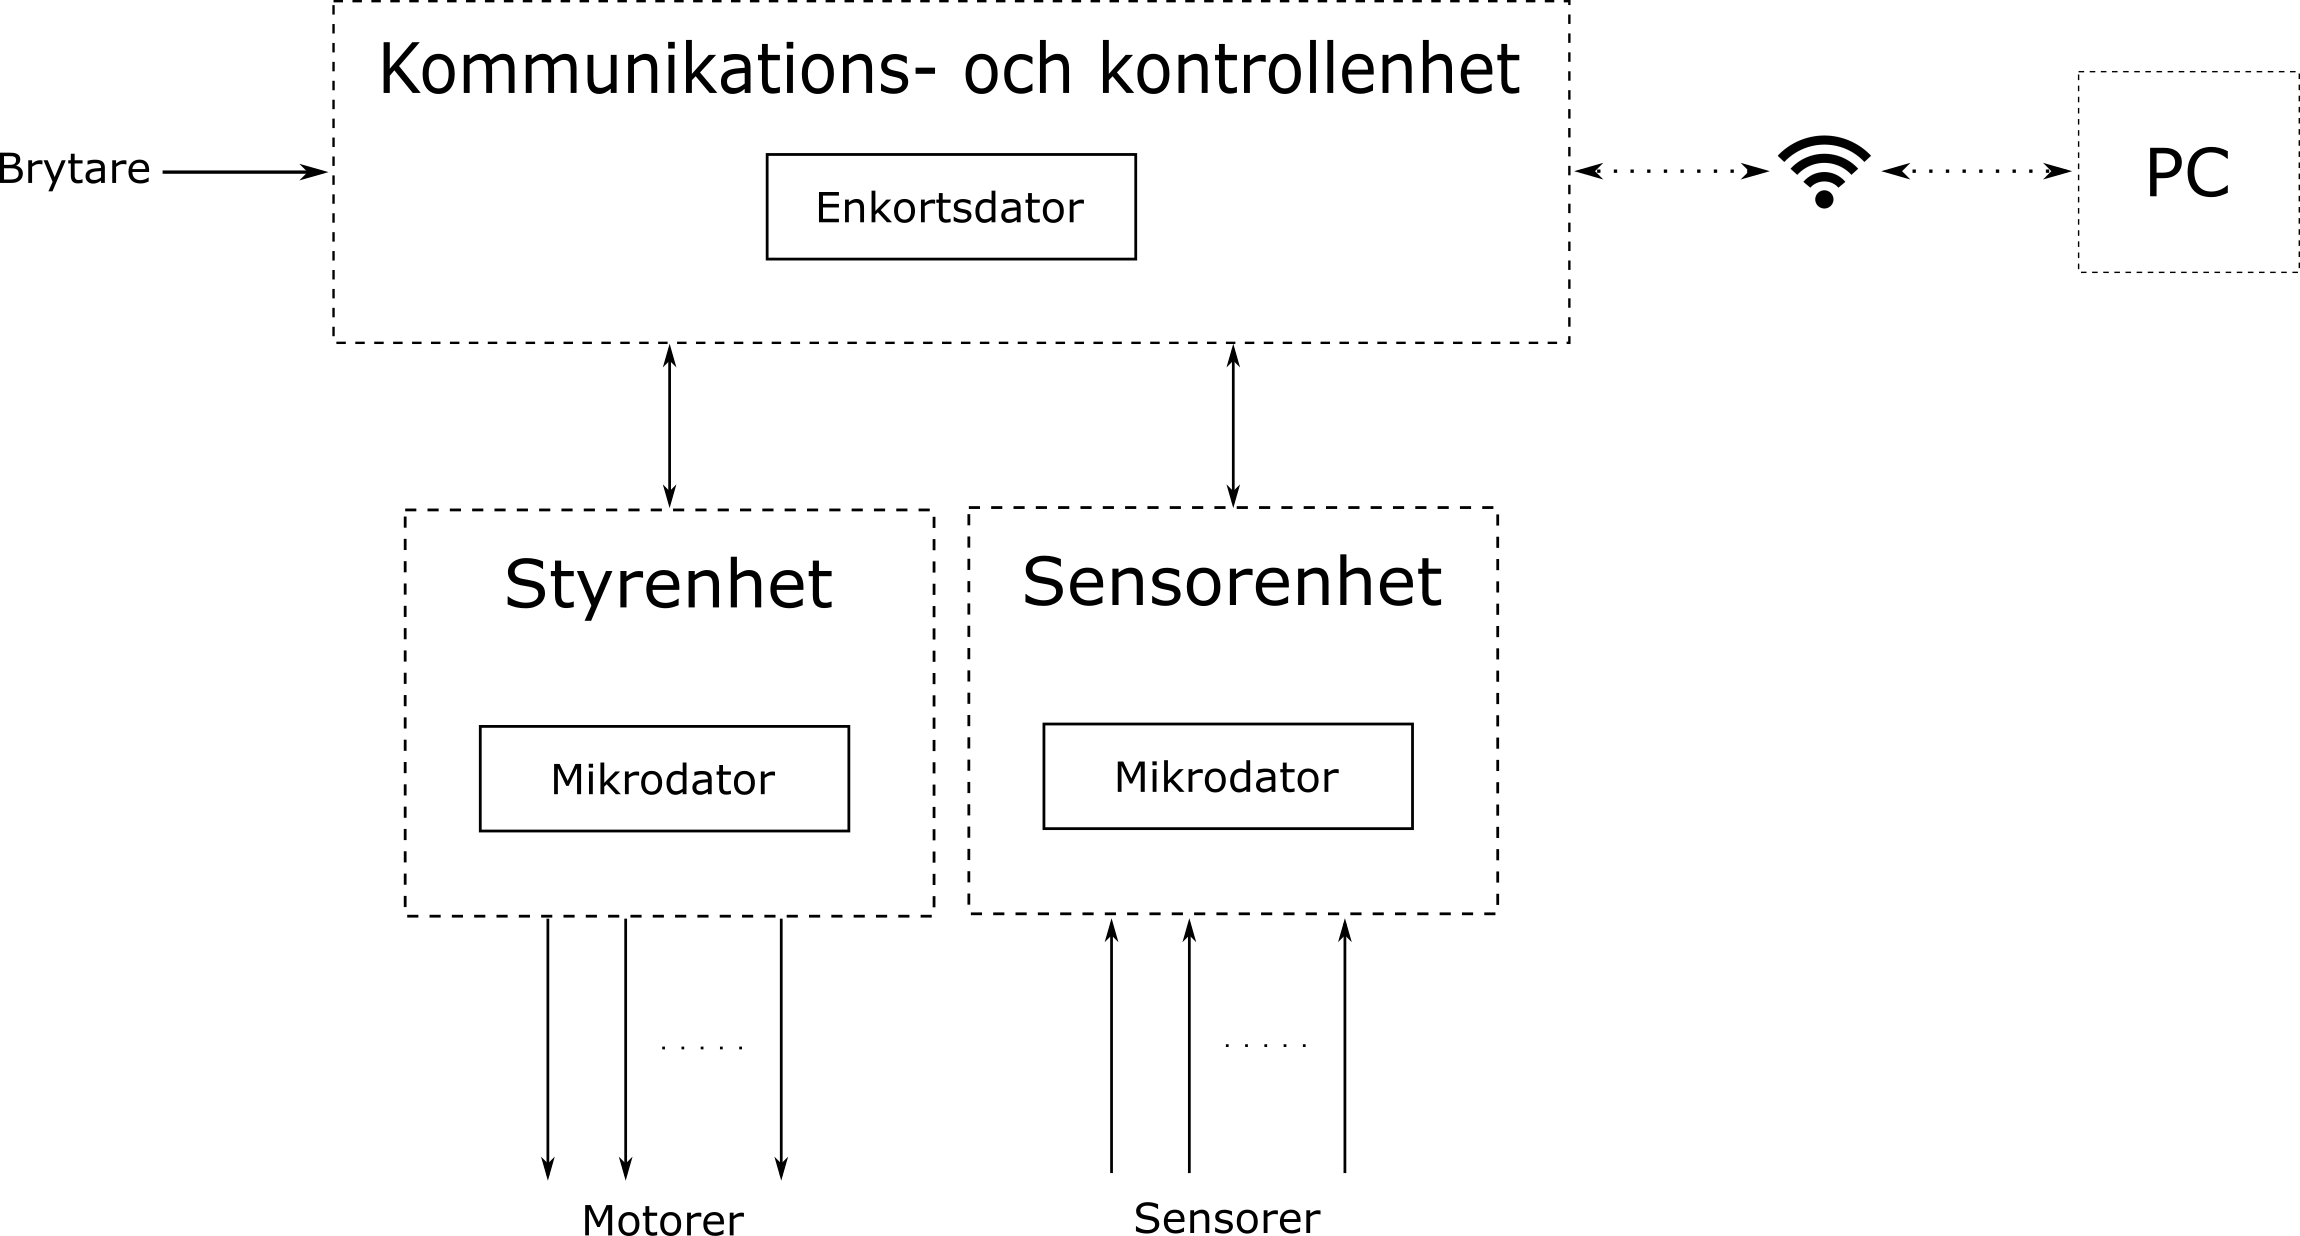
\includegraphics[width=1\textwidth]{modules.png}}
    \caption{Modulöversikt.}
    \label{fig:modules}
\end{figure}

Robotens hårdvara är monterad ovanpå dess chassi, en modell som går under namnet \cite{terminator}. Denna kommer med fyra hjul påmonterade, som används för att roboten ska kunna ta sig runt i rummet. Ytterligare ett servo, monteras på toppen av roboten.

Ovanpå denna sitter den avståndskänsliga lasern LIDAR - systemets viktigaste sensor vad gäller rumskanningen. Ytterligare sensorer hittas på tre av robotens fyra sidor: IR-sensorer för bättre kontroll under körning. Ingen sensor är monterad längst fram på chassit, eftersom LIDAR:n täcker den funktionaliteten då roboten rör på sig.

Vidare är ett ett gyro (modell MPU6050) monterat i mitten av roboten för att den ska kunna rotera mer precist.

I bilaga \ref{app:placement} hittas en grafisk beskrivning av hårdvarans placering. Kopplingsscheman finns i bilaga \ref{schematics:styrenhet} till och med bilaga \ref{schematics:brain}.


\subsection{Kommunikation}
\label{ssec:communication}

\subsection{Seriell kommunikation}
För kommunikation mellan kommunikation- och kontrollenheten (se kapitel \ref{sec:system3}) och sensorenheten samt styrenheten (se kapitel \ref{sec:system2} respektive \ref{sec:system3}) används seriella bussar. Då Raspberry pi:n som används i kontrollenheten saknar användbar inbyggd UART så används USB-till-UART-moduler. Den seriella kommunikationen körs med en baud rate på $38 400$.

Alla meddelanden (instruktioner såväl som svar) påbörjas med ett metapaket på 8 bitar som följs av noll eller flera datapaket som illustrerat i figur \ref{fig:msg_structure}. Se tabell \ref{tab:meta_packet} för en mer ingående förklaring över fälten i metapaketet.

\begin{figure}[h!]
\centering
\begin{bytefield}[bitwidth=30pt,bitformatting={\small\bfseries}]{8}
\bitheader{0-7} \\
\begin{rightwordgroup}{Metapaket}
\bitbox{1}{\footnotesize Adress} & \bitbox{3}{Längd} & \bitbox{4}{Typ}
\end{rightwordgroup} \\
\begin{rightwordgroup}{\textit{Längd} stycken datapaket}
\wordbox[lrt]{1}{Data} \\
\skippedwords \\
\wordbox[lrb]{1}{}
\end{rightwordgroup} \\
\end{bytefield}

\caption{Ett meddelande.}
\label{fig:msg_structure}
\end{figure}

\begin{table}[h]
    \centering
    \rowcolors{2}{gray!25}{white}
    \begin{tabular}{|l|l|l|}
        \rowcolor{gray!50}
        \hline
        \textbf{Bitar} & \textbf{Namn} & \textbf{Betydelse} \\ \hline
        \texttt{0} & Adress & 0 motsvarar styrenhet, 1 motsvarar sensorenhet. \\
        \texttt{1-3} & Storlek & Antal paket med argument som följer metapaketet. \\
        \texttt{4-7} & Typ & Vilken typ av kommando/svar som skickas. \\ \hline
    \end{tabular}
    \caption{Metapaketets utformning.}
    \label{tab:meta_packet}
\end{table}

% TODO: Skriv om acknowledge.

\subsubsection{Kontrollenhet $\leftrightarrow$ Styrenhet} \label{sssec:kontrollenhet_arrow_styrenhet}
\label{sec:controlCommunication}
% TODO: Fixa upplägget med sektioner
\paragraph{Drive}
\texttt{Drive}-instruktionen kör roboten framåt eller bakåt enligt argumenten som beskrivs i tabell \ref{tab:drive}. Kommandot har typnummer \texttt{1}.
\begin{table}[h!]
    \centering
    \rowcolors{2}{gray!25}{white}
    \begin{tabular}{|l|l|L{300pt}|}
    \rowcolor{gray!50}
    	\hline
    	\textbf{Argument} & \textbf{Storlek (bytes)} & \textbf{Betydelse} \\ \hline
    	\texttt{Direction} & 1 & 0 motsvarar framåt, 1 bakåt. \\
    	\texttt{Speed} & 1 & Integer mellan 0 och 100, där 100 är maxhastighet och 0 stillastående. \\
    	\texttt{Time} & 2 & Integer i millisekunder. 16 bitar uppdelat på (först) höga 8 bitar och sedan låga 8 bitar. \\ \hline
    \end{tabular}
    \caption{\texttt{Drive}-instruktionens argument.}
    \label{tab:drive}
\end{table}

\paragraph{Turn}
\texttt{Turn}-instruktionen svänger roboten enligt argumenten som beskrivs i tabell \ref{tab:turn}. Kommandot har typnummer \texttt{2}.
\begin{table}[h!]
    \centering
    \rowcolors{2}{gray!25}{white}
    \begin{tabular}{|l|l|L{300pt}|}
    \rowcolor{gray!50}
    	\hline
    	\textbf{Argument} & \textbf{Storlek (bytes)} & \textbf{Betydelse} \\ \hline
    	\texttt{Direction} & 1  & 0 motsvarar vänster, 1 höger. \\
    	\texttt{Speed} & 1 & Integer mellan 0 och 100, där 100 är maxhastighet och 0 stillastående. \\
    	\texttt{Time} & 2 & Integer i millisekunder. 16 bitar uppdelat på (först) höga 8 bitar och sedan låga 8 bitar. \\ \hline
    \end{tabular}
    \caption{\texttt{Turn}-instruktionens argument.}
    \label{tab:turn}
\end{table}

\paragraph{Side-speed}
\texttt{Side-speed}-instruktionen sätter vänster och höger motorpar enligt argumenten som beskrivs i tabell \ref{tab:side_speeds}. Kommandot har typnummer \texttt{3}.
\begin{table}[h!]
    \centering
    \rowcolors{2}{gray!25}{white}
    \begin{tabular}{|l|l|L{250pt}|}
    \rowcolor{gray!50}
    	\hline
    	\textbf{Argument} & \textbf{Storlek (bytes)} & \textbf{Betydelse} \\ \hline
    	\texttt{Left direction} & 1 & 0 motsvarar framåt, 1 bakåt. \\
    	\texttt{Left speed} & 1 & Integer mellan 0 och 100, där 100 är maxhastighet och 0 stillastående. \\
    	\texttt{Right direction} & 1 & 0 motsvarar framåt, 1 bakåt. \\
    	\texttt{Right speed} & 1 & Integer mellan 0 och 100, där 100 är maxhastighet och 0 stillastående. \\ \hline
    \end{tabular}
    \caption{\texttt{Side-speeds}-instruktionens argument.}
    \label{tab:side_speeds}
\end{table}


\paragraph{Servo}
\texttt{Servo}-instruktionen sätter servot till en specificerad vinkel enligt argumentet som beskrivs i tabell \ref{tab:servo}. Kommandot har typnummer \texttt{4}.
\begin{table}[h!]
    \centering
    \rowcolors{2}{gray!25}{white}
    \begin{tabular}{|l|l|l|}
    \rowcolor{gray!50}
    	\hline
      \textbf{Argument} & \textbf{Storlek (bytes)} & \textbf{Betydelse} \\ \hline
      \texttt{Direction} & 1 & Servots vinkel, mellan 0 och 180 \\ \hline
    \end{tabular}
    \caption{\texttt{Servo}-instruktionens argument.}
    \label{tab:servo}
\end{table}

\paragraph{Stop-Motors}
\texttt{Stop-motors}-instruktionen stannar båda motorerna. Kommandot har typnummer \texttt{5}.

\paragraph{Controller-Information}
\texttt{Controller-Information}-instruktionen ber styrenheten om diagnostisk data som returneras såsom specificerat i tabell \ref{tab:controller_information}. Kommandot har typnummer \texttt{6}.


\begin{table}[h!]
    \centering
    \rowcolors{2}{gray!25}{white}
    \begin{tabular}{|l|l|L{250pt}|}
    \rowcolor{gray!50}
    	\hline
    	\textbf{Argument} & \textbf{Storlek (bytes)} & \textbf{Betydelse} \\ \hline
    	\texttt{Left direction} & 1 & 0 motsvarar framåt, 1 bakåt. \\
    	\texttt{Left PWM}  & 1 & Integer mellan 0 och 255, där 255 är maxhastighet och 0 stillastående. \\
    	\texttt{Right direction} & 1 & 0 motsvarar framåt, 1 bakåt. \\
    	\texttt{Right PWM} & 1 & Integer mellan 0 och 255, där 255 är maxhastighet och 0 stillastående. \\
    	\texttt{Servo PWM} & 2 & Integer mellan 0 och 65535, där 773 är längst till vänster och 2343 till höger. \\ \hline
    \end{tabular}
    \caption{Returvärden från \texttt{Controller-Information}-instruktionen.}
    \label{tab:controller_information}
\end{table}

\subsubsection{Kontrollenhet $\leftrightarrow$ Sensorenhet}
\paragraph{Read-IR}
\label{sec:sensorCommunication}
IR-sensorer läses av med typnummer enligt tabell \ref{table:irtypes} och returneras såsom specificerat i tabell \ref{tab:ir}.

\begin{table}[h!]
    \centering
    \rowcolors{2}{gray!25}{white}
    \begin{tabular}{|l|l|}
    \rowcolor{gray!50}
    	\hline
    \textbf{Typnummer} & \textbf{Sensor} \\ \hline
    \texttt{1} & Vänster fram \\
    \texttt{2} & Vänster bak \\
    \texttt{3} & Höger fram \\
    \texttt{4} & Höger bak  \\
    \texttt{5} & Bak \\ \hline
    \end{tabular}
    \caption{Typvärden för IR-avläsning.}
    \label{table:irtypes}
\end{table}


\begin{table}[h!]
    \centering
    \rowcolors{2}{gray!25}{white}
    \begin{tabular}{|l|l|l|}
    \rowcolor{gray!50}
    	\hline
    	\textbf{Argument} & \textbf{Storlek (bytes)} & \textbf{Betydelse} \\ \hline
    	\texttt{Avstånd} & 2 & Integer mellan 0 och 300. Avstånd i millimeter \\ \hline
    \end{tabular}
    \caption{Returvärden från IR-avläsning.}
    \label{tab:ir}
\end{table}

\paragraph{Read-Lidar}
Läser av LIDAR-sensorn och returneras dess värde såsom specificerat i tabell \ref{tab:lidar}. Kommandot har typnummer \texttt{6}.
\begin{table}[h!]
    \centering
    \rowcolors{2}{gray!25}{white}
    \begin{tabular}{|l|l|l|}
    \rowcolor{gray!50}
        \hline
        \textbf{Argument} & \textbf{Storlek (bytes)} & \textbf{Betydelse} \\ \hline
        \texttt{Avstånd} & 1 & Integer mellan 0 och 65535. Avstånd i millimeter \\ \hline
        \end{tabular}
    \caption{Returvärden från LIDAR-avläsning.}
    \label{tab:lidar}
\end{table}


\paragraph{Read-Gyro}
Läser av gyrots X-axel, vilket motsvaras av robotens z-axel, och returneras dess värde såsom specificerat i tabell \ref{tab:gyro}. Kommandot har typnummer \texttt{7}.
\begin{table}[h!]
    \centering
    \rowcolors{2}{gray!25}{white}
    \begin{tabular}{|l|l|l|}
    \rowcolor{gray!50}
        \hline
        \textbf{Argument} & \textbf{Storlek (bytes)} & \textbf{Betydelse} \\ \hline
        \texttt{Avstånd} & 2 & Integer mellan -25206 och 25205. Vinkelhastighet i centigrader/s. \\ \hline
    \end{tabular}
    \caption{Returvärden från gyro-avläsning.}
    \label{tab:gyro}
\end{table}

\subsection{WIFI-kommunikation}
Kommunikation- och kontrollenheten kommunicerar via Wi-Fi med PC-mjukvaran (se kapitel \ref{sec:system4}). Då programmet körs ansluter kontrollenheten till \texttt{eduroam} och annonserar sin IP-adress till gruppens Slack-kanal. Därefter kan PC-mjukvaran ansluta till denna IP-adress. Detta sker via en socket, där kontrollenheten är server och PC-mjukvaran klient.

Kommandon skickas som strängar. När större data, som argument, behövs, så skickas dessa som ett JSON-objekt. Följande kommandon finns tillgängliga:

\begin{description}
    \item [TRANSMIT] Utför nästa UART-command som skickas.
    \item [FORWARD\_MOTOR\_INFO] Svara med motorenhetsdata (\texttt{dict}), kodat med JSON.
    \item [FORWARD\_SENSOR\_INFO] Svara med sensorenhetsdata (\texttt{dict}), kodat med JSON.
    \item [KEY\_EVENT] Om vi är i det manuella läget: uppdatera motorstyrning med skickad tangent. Tangenten som skickas därefter är en sträng som innehåller ''\texttt{left}'', ''\texttt{right}'', ''\texttt{up}'', eller ''\texttt{down}''.
    \item [SEND\_MAP] Svara med kartan, så som den ser ut för tillfället. Kartan är en två-dimensionell lista med 1:or och 0:or, kodad med JSON.
    \item [TOGGLE\_MODE] Om vi är i det manuella läget: byte till autonomt. Annars: byt till manuellt.
\end{description}


\clearpage
\section{Sensorenhet} \label{sec:system1}
Sensorenheten har i uppgift att läsa in sensordata och omvandla den till ett läsligt format. Den innehåller en processor av modellen ATmega1284, 5 IR-sensorer, en lasersensor, 2 reflex sensorer, samt gyro.

IR-sensorerna används för navigering - bland annat ger de indata till reglerings algoritmen: väggavstånd. Lasersensorn, LIDAR, används för skanning av rummet. Med hjälp av gyrot kan vi se till att vi utför våra 90-graders-svängar korrekt. De 2 reflex sensorerna sitter på hjulen och används för att avgöra hur långt vi har kört.

Se figur \ref{fig:unitSensor} för en övergripande systemskiss för sensorenheten.

\begin{figure}[h!]
	\makebox[\textwidth][c]{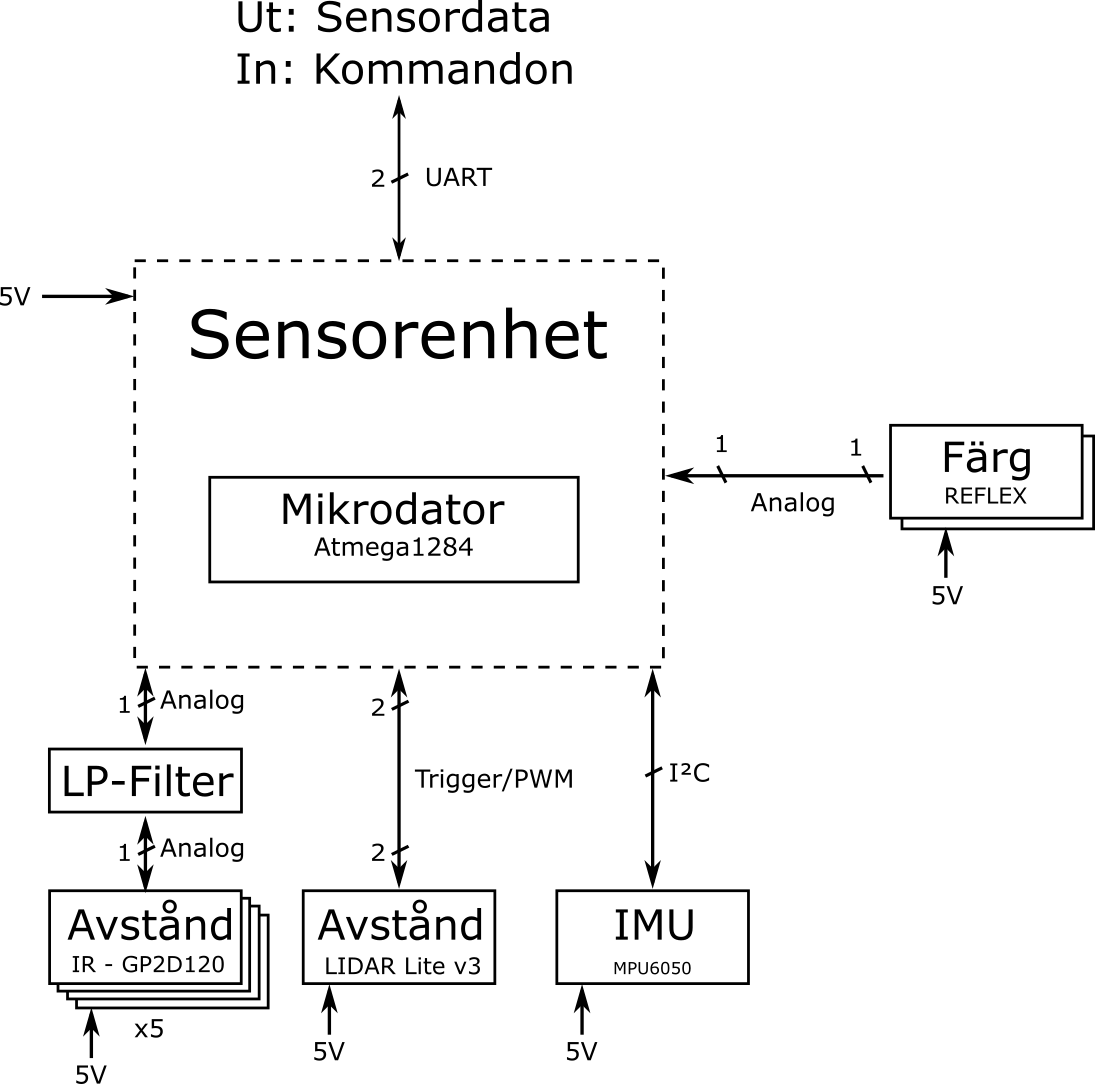
\includegraphics[width=0.9\textwidth]{sensorenhet.png}}
	\caption{Översikt över sensorenheten.}
	\label{fig:unitSensor}
\end{figure}

\clearpage

\subsection{Hårdvara}

\subsubsection{Processor}
ATmega1284 används som processormodell, då den är kraftfull utan att ta det är till överdrift. Antalet pinnar, A/D-omvandlare, interrupts samt UART-enheter som processorn har räcker för samtliga sensorer och kommunikationsbussar.

\subsubsection{IR-sensorer} \label{sssec:sonicsensors}
Det placeras två stycken IR-sensorer av modell GP2D120 på både höger och vänster sida om roboten (för totalt fyra), samt en på baksidan. För avståndsmätning framåt används LIDARn. Se bilaga \ref{app:placement} för sensorernas placacering på roboten. Dessa sensorer används för navigering och positionsuppskattning. Med hjälp av de dubbla IR-sensorerna på vardera sida kan det avgöras ifall roboten åker parallellt med väggen. Dessa behöver en A/D-omvandlare var, som är inbyggd i processorn ATmega1284. Se kapitel \ref{ssec:sensorInterface}. Sensorerna kan effektivt mäta avstånd inom intervallet 4 till 30 cm vilket räcker, då roboten är tänkt att följa en vägg och köra inom ett rutnät, där varje ruta är 40x40cm.

\subsubsection{LP-filter}
De sensorer som skickar en analog signal kommer att få med sig endel brus, vilket kan medföra att mätvärdena får stora avvikelser. För att få bort detta brus så är sensorer med analoga signaler (förrutom reflex sensorer) kopplade till LP-filter som filtrerar bort frekvenser över ungefär 88 Hz. Referenssignalen som AD-omvandlarna använder har också ett LP-filter då det förbättrar noggranheten i avläsningen i ATmega:n betydligt.

\begin{figure}[h!]
	\makebox[\textwidth][c]{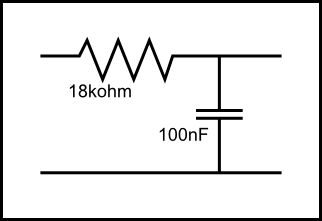
\includegraphics[width=0.3\textwidth]{lp-filter.png}}
	\caption{LP-filtrets konstruktion.}
	\label{fig:lpFilter}
\end{figure}

\subsubsection{LIDAR} \label{sssec:lidar}
LIDAR är en lasersensor som används för rumsavskanning. Vi kommunicerar med komponenten via en trigger-pin; tiden som signaler är höga är linjära gentemot uppmätt avstånd. Vi använder även denna för att se om vi håller på att köra in i en vägg.

Sensorn monteras på toppen av roboten - ovanpå ett roterande servo, som specificeras i större detalj i kapitel \ref{ssec:servomotor}. Detta för att kunna mäta avstånd i flera vinklar (0 till 180 grader) utan att rotera roboten.

\subsubsection{Gyro} \label{sssec:imu}
MPU6050 är ett gyro som används via en I2C-bus. Den ger oss rotationen kring z-axeln, som användas för att beräkna robotens riktning i rummet under svängar. Gyrot läses endast av när det efterfrågas (under sväng).

\subsubsection{Reflex sensorer}
Reflex sensorerna skickar ut en analog signal som varierar beroende på hur mycket ljus som avges från ytan den siktar på. Eftersom att de två bakre hjulen har en färgskala påklistrad som skiftar mellan svart och vit kommer signalen att pendla mellan två olika spänningar. Varje färg består i 1/8 av ett varv, vilket betyder att när reflex sensorerna ändrat signalstyrkan så vet vi att hjulet snurrat 1/8 av ett varv. På detta sätt kan vi räkna ut hur långt roboten har kört.

\subsubsection{Komponentbudget}
Här följer en lista på all hårdvara som detta delsystem kräver.

\begin{HardwareList}
\hardware{ATmega1284}{Mikroprocessor med 40 pinnar (inklusive 8 A/D-omvandlare).}{1}
\hardware{EXO-3}{Oscillator för ATmega-klockan, med standardfrekvens \SI{16}{\mega\hertz}. Körs i \SI{8}{\mega\hertz}}{1}
\hardware{GP2D120}{IR-sensor.}{5}
\hardware{Resistor}{Till LP-filter. \SI{18}{\kilo\ohm}}{6}
\hardware{Kondensator}{Till LP-filter. \SI{100}{\nano\farad}}{6}
\hardware{LIDAR lite v3}{Avancerad lasersensor.}{1}
\hardware{Resistor}{Separation av trigger och monitor för LIDAR. \SI{1}{\kilo\ohm}}{1}
\hardware{Kondensator}{Störningsreducering av LIDAR. \SI{680}{\micro\farad}.}{1}
\hardware{MPU6050}{Gyro/Accelerometer.}{1}
\hardware{Reflex sensor}{Detekterar färgändringar på hjulet. Används till att räkna ut hur långt vi kört.}{2}
\end{HardwareList}

\subsection{Mjukvara}

Koden skrivs i C, och ska följa standarden specificerad i bilaga \ref{sec:cstandard}.

På instruktion läser sensorenheten av en sensor för att sedan skicka vidare värdet på ett mer lättanvänt format (se kapitel \ref{ssec:sensorInterface}) samt tar emot instruktioner om att läsa av en viss sensor. För IR-sensorer beräknas ett medelvärde över de senaste fem mätningarna (då dess utvärden kan vara avvikande), medan övriga sensorvärden skickas tillbaka direkt.

\subsection{Gränssnitt} \label{ssec:sensorInterface}
Sensorenheten ska kommunicera med alla sensorer och skicka vidare utdata. Mer information om interenhetskommunikationen finner man i kapitel \ref{sssec:kontrollenhet_arrow_styrenhet}.

% TODO: Mer om protokollen till hårdvaran
% Om vi inte tar bort denna sektionen; protokollen är typ beskrivna nedan ändå.

\subsubsection{LIDAR}
LIDAR kommer använda avläsningstriggers och PWM via en gemensam pin på sensorn. På ATmega-sidan delas denna upp i två pinnar med en resistor på triggersignalen som gör att LIDARns signaler får prioritet. PWM-signalen är kopplad till ett avbrott för att mäta dess längd, som används för att beräkna avståndet i millimeter.

\clearpage

\subsubsection{Gyro}
MPU6050 läses av via I2C. Endast gyrot i robotens z-axel används, vilket motsvaras av gyrons x-axel (då det inte ligger plant gentemot chassit). Mätvärdeskalibrering med hjälp av temperatursensorn på gyrot används ej. Dock så beräknar sensorenheten gyrots drift-hastighet vid start och kalibrerar för det. Gyrot är inställt på att använda en maximal vinkelhastighet på 250 grader/s. Efter avläsning omvandlas vinkelhastigheten till centigrader/s.

\subsubsection{Reflex sensorer}
Reflex sensorerna skickar en analog signal till AD-omvandlarna. Eftersom att spänningen skljer sig ganska mycket beroende på om reflex sensorn pekar på en svart eller vit yta så behöver vi inget LP-filter här.

För varje gång som reflex sensorn detekterar att färgen skiftat från svart till vit eller tvärtom så adderar ATmega:n 1 till respektive räknare. På detta sätt kan vi räkna ut hur långt ett hjul har snurra.

\subsubsection{IR-sensorer}
IR-sensorerna använder en analog utgång som varierar i enlighet med avståndet efter en ickelinjär kurva. Denna signal har störningar som filtreras ut med hjälp av LP-filter, se kopplingsschema i bilaga \ref{schematics:styrenhet}. Efter avläsning i form av spänningen, $v$, som går mellan 0 och 5 volt översätts detta med formeln $d = 10 \times (v/4.577) ^{(1/-0.634)}$ till ett avstånd, $d$, i millimeter.

\subsubsection{Utvärden/Input}
En seriell buss via den inbyggda UART-hårdvaran används. Via denna buss tas avläsningsinstruktioner emot och sensordata skickas, enligt kapitel \ref{sec:sensorCommunication}.

\clearpage
\section{Styrenhet} \label{sec:system2}
Styrenheten är ansvarig för robotens lågnivåstyrning. Den är länken mellan alla styrkommandon och motorer. Se figur \ref{fig:unitMotorcontroller} för en övergripande systemskiss för styrenheten.

\begin{figure}[h!]
    \makebox[\textwidth][c]{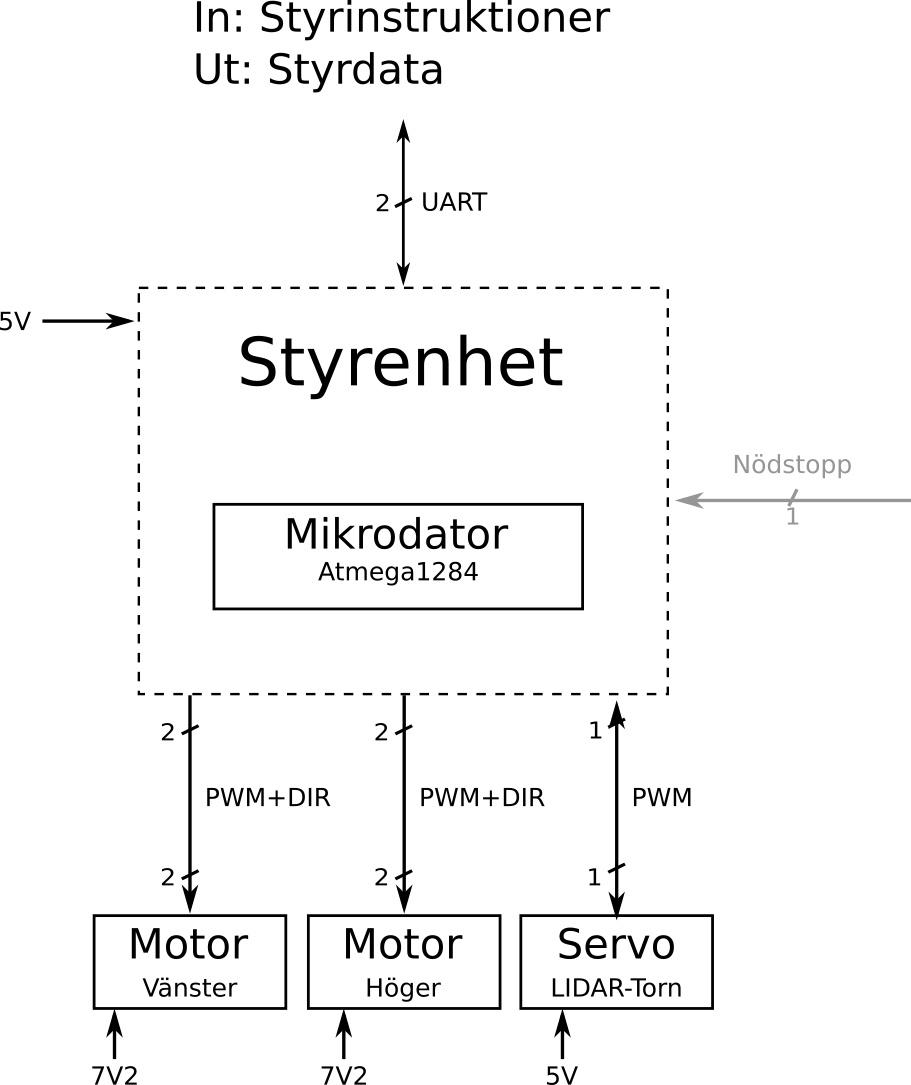
\includegraphics[width=0.6\textwidth]{styrenhet.png}}
    \caption{Översikt över styrenheten.}
    \label{fig:unitMotorcontroller}
\end{figure}

\subsection{Hårdvara}

\subsubsection{Processor}
Vi använder en ATmega1284-processor för styrmodulen. Processorn kommunicerar med 4 DC-motorer som sitter på chassit (\cite{terminator}) och ett servo. Alla motorer styrs med PWM.

\clearpage

\subsubsection{Servo/steppermotor} \label{ssec:servomotor}
På toppen av roboten ska en lasersensor (se kapitel \ref{sssec:lidar}) vara monterad, ovanpå en servo som tillåter sensorn att rotera. Servomotorn är ett hobbyservo.

Hobbyservot styrs med PWM. Svängvidden är 180 grader. Styrenheten tar emot styrsignaler på engradersnivå, och räknar om det till en PWM-signal.

\subsubsection{Hjulmotorer}
Totalt är det fyra motorer som är monterade på chassit. De fyra DC-motorerna styrs parvis (höger sida och vänster sida) med hjälp av en PWM-signal samt en rotationsriktningssignal per motorpar. Sammanlagt används alltså 4 pinnar på processorn för styrning av hjulen. Styrenheten tar emot hastigheter via seriella kommandon enligt kapitel \ref{sec:controlCommunication} och omvandlar dessa till PWM-signaler.

\subsubsection{Komponentbudget}
Här följer en lista på all hårdvara som detta delsystem kräver.

% TODO add hardware
\begin{HardwareList}
\hardware{ATmega1284}{Mikroprocessor med 40 pinnar (inklusive 8 A/D-omvandlare).}{1} 
\hardware{EXO-3}{Oscillator för ATmega-klockan, med standardfrekvens \SI{16}{\mega\hertz}. Körs i \SI{8}{\mega\hertz}}{1}
\hardware{Hobbyservo}{Används för att snurra på LIDAR lasern.}{1}
\hardware{Terminator}{Chassi som roboten är byggd på.}{1}
\hardware{DC-motor}{Är monterat på Terminator chassit.}{4}
\end{HardwareList}

\subsection{Mjukvara}
Koden skrivs i C, och ska följa standarden specificerad i bilaga \ref{sec:cstandard}. 

\clearpage

\subsubsection{Tillståndsdiagram}
Som vi ser i tillståndsdiagrammet för styrenheten (figur \ref{fig:stateDiagram}) så har vi totalt tre olika tillstånd. Medan styrenheten är i tillståndet \texttt{WAIT} så kommer roboten att stå stilla och invänta en instruktion. Notera att en instruktion kan sättas i alla tillstånd, så om roboten redan har en instruktion inläst då tillståndet sätts till \texttt{WAIT} så kommer roboten börja på denna instruktion omedelbart utan att stanna.

\begin{figure}[h!]
	\makebox[\textwidth][c]{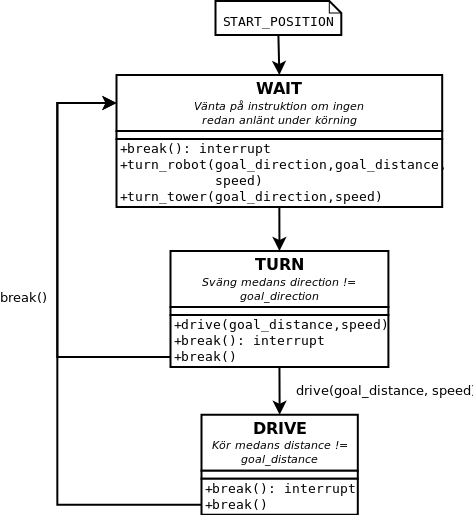
\includegraphics[width=0.5\textwidth]{styrenhet-statediagram.png}}
	\caption{Tillståndsdiagram för styrenheten.}
	\label{fig:stateDiagram}
\end{figure}

\clearpage

\subsubsection{Övergripande programflöde}
I flödesschemat i figur \ref{fig:styrenhetFlowchart} ser vi att det finns funktionalitet som inte avslöjade sig i tillståndsdiagrammet, det vill säga hur vi hanterar de olika instruktionerna \texttt{SCAN} och \texttt{DRIVE}. Om instruktionen är av typen \texttt{SCAN} så kommer aldrig styrenheten att gå in i tillståndet \texttt{TURN} då det inte finns något avstånd att köra. Denna typ av design utesluter givetvis möjligheten att köra och scanna samtidigt. För mer information angående vad de lika instruktionstyperna står för, se kapitel \ref{ssec:controlInterface}. 

\begin{figure}[h!]
\centering
\begin{tikzpicture}[node distance=2cm,scale=0.6, every node/.style={scale=0.6}]
% Styles
\tikzstyle{startstop} = [rounded rectangle, minimum width=3cm, minimum height=1cm,text centered, draw=black, fill=red!30, align=center, inner sep=10pt]
\tikzstyle{io} = [trapezium, trapezium left angle=70, trapezium right angle=110, minimum width=3cm, minimum height=1cm, text centered, draw=black, fill=blue!30, align=center, inner sep=10pt]
\tikzstyle{process} = [rectangle, minimum width=3cm, minimum height=1cm, text centered, draw=black, fill=orange!30, align=center, inner sep=10pt]
\tikzstyle{decision} = [diamond, minimum width=3cm, minimum height=1cm, text centered, draw=black, fill=green!30, align=center, inner sep=10pt, aspect=2]
\tikzstyle{arrow} = [thin,->,>=stealth]

\node (start) [startstop] {Start};
\node (wait_state) [process, below of=start] {\texttt{WAIT\_STATE\_ACTIVATED}};
\node (is_instruction_ready) [decision, right of=wait_state, xshift=6cm] {Any instruction ready \\ to be executed?};
\node (brake) [process, right of=is_instruction_ready, xshift=6cm] {Stop motors};
\node (turn_state) [process, below of=is_instruction_ready, yshift=-2cm] {\texttt{TURN\_STATE\_ACTIVATED} \\ \\ Turn robot/tower to \\ \texttt{goal\_direction}};
\node (scan_or_drive) [process, below of=turn_state, yshift=-1cm] {Is instruction \texttt{SCAN} or \texttt{DRIVE}?};
\node (drive_state) [process, below of=scan_or_drive, yshift=-0.8cm] {\texttt{DRIVE\_STATE\_ACTIVATED} \\ \\ Drive distance \texttt{goal\_distance}};

\draw [arrow] (start) -- (wait_state);
\draw [arrow] (wait_state) -- (is_instruction_ready);
\draw [arrow] (is_instruction_ready) -- node[auto] {No} (brake);
\draw [arrow] (is_instruction_ready) -- node[auto] {Yes} (turn_state);
\draw [arrow] (turn_state) -- (scan_or_drive);
\draw [arrow] (scan_or_drive) -- node[auto] {\texttt{DRIVE}} (drive_state);
\draw [arrow] (scan_or_drive) -| node[anchor=south, xshift=4cm] {\texttt{SCAN}} (wait_state);
\draw [arrow] (drive_state) -| (wait_state);

\coordinate[above of=is_instruction_ready, yshift=1cm] (d0);
\draw [-] (brake) |- (d0);
\draw [arrow] (d0) -- (is_instruction_ready);


\end{tikzpicture}
	%\makebox[\textwidth][c]{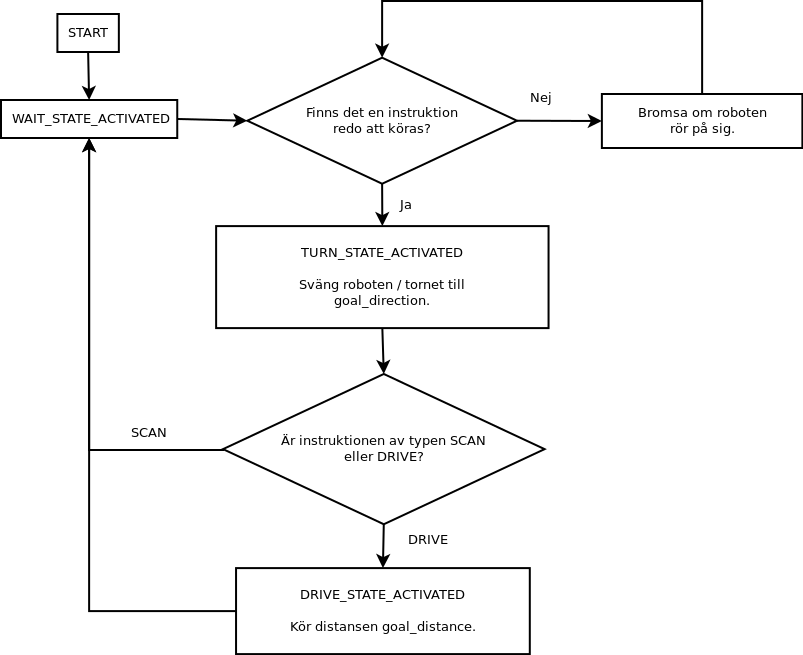
\includegraphics[width=0.9\textwidth]{styrenhet-flowchart.png}}
	\caption{Flödesschema för styrenheten.}
	\label{fig:styrenhetFlowchart}
\end{figure}

\subsubsection{Processer}
Eftersom att hårdvaran sköter inläsning från en pinne parallellt med det program som körs så behövs inte mer än en process för styrenheten.

\clearpage

\subsection{Gränssnitt} \label{ssec:controlInterface}

\subsubsection{Styrsignaler samt styrdata}
Vi implementerar en seriell buss som går mellan styrenheten och kommunikationsenheten.

Styrdatan ska innehålla information om följande punkter:
\begin{itemize}
	\item Om instruktionen är av typen \texttt{SCAN} eller \texttt{DRIVE}. \texttt{SCAN} styr servot medans \texttt{DRIVE} styr DC motorerna.
	\item Hur många grader roboten/servot ska rotera.
	\item Hur långt roboten ska köra i den givna riktningen. Denna information är endast intressant om instruktionen är av typen \texttt{DRIVE}.
	\item Vilken hastighet de givna motorerna ska köra med.
\end{itemize}

Från styrenheten skickas information om vilka hastigheter motorerna/servot fått när instruktionen utförs.

\clearpage
\section{Kommunikations- och kontrollenhet} \label{sec:system3}
Kommunikations- och kontrollenheten agerar som en central hjärna i systemet. Den tar emot data från de andra delsystemen, och gör val som bidrar till att systemets funktionalitet som helhet uppfylls.

Inga andra delsystem kommunicerar direkt med varandra, utan endast med kommunikations- och kontrollenheten. Se figur \ref{fig:unitBrain} för en övergripande skiss.

%TODO: Lägg till knappar som går till PI:n i schemat
\begin{figure}[h!]
    \makebox[\textwidth][c]{
\includegraphics[width=1\textwidth]{brain.png}}
    \caption{Översikt över kommunikations- och kontrollenheten.  }
    \label{fig:unitBrain}
\end{figure}

\subsection{Hårdvara}

\subsubsection{Datormodell}
Raspberry Pi 3 används, med inbyggd Wi-Fi-modul. Denna lilla dator är relativt kraftig, och bör därmed inte ha problem med att hålla sitt program gående i rimlig takt. Antalet portar räcker också till: två USB-utgångar behövs för USB-UARTen och två pinnar behövs för brytare och reset-signal (se kapitel \ref{ssec:brainInterface}).

Då enkortsdatorn kan korrumpera SD-kortet vid brytning av strömmen så finns en knapp med funktionen att stänga ner mjukvaran. Denna används då lämpligen innan brytaren för strömmen.

För strömförsörjning används en USB-kabel från robotplatformen.

\subsubsection{Komponentbudget}
Här följer en lista på all hårdvara som detta delsystem använder.

\begin{HardwareList}
\hardware{Raspberry Pi 3}{Enkortsdator.}{1}
\hardware{SD-kort}{SD-kort på minst 4GB används som lagringsenhet.}{1}
\hardware{Avstudsad tryckknapp}{För nedstängning av mjukvara.}{1}
\hardware{Avstudsad tryckknapp}{För byte av styrläge.}{1}
\end{HardwareList}

\subsection{Mjukvara}
Koden skrivs i Python 3, och ska följa \cite{pep8}. Operativsystemet som används är Raspbian.

\subsubsection{Kommunikation}
Delsystemet är vad som i slutändan kontrollerar de olika delsystemen, och måste därför kunna skicka meddelanden mellan dessa. Mjukvara skrivs för att kunna skicka meddelanden över de olika gränssnitten som den kopplas upp emot (se kapitel \ref{ssec:brainInterface}).

Förutom hårdvarugränssnitt ska den också kunna kommunicera med en extern PC (se kapitel \ref{sec:system4}) med hjälp av Wi-Fi-kommunikation, där den kontinuerligt skickar debugdata och kartinformation samt tar emot meddelanden. Dessa meddelanden behandlas i den ordning de köats i pc-mjukvaran och används för att antingen byta läge på roboten, eller för att ge kommandon under manuell styrning. Mjukvaran för Wi-Fi-kommunikationen skrivs och ligger som en egen tråd för att utgöra mjukvarukomponenten i kommunikationsmodulen. För en illustration över hur Wi-Fi-kommunikationen fungerar, se figur \ref{fig:wifi}.

% TODO implementeras UART m.h.a avbrott?
% TODO olika köer för meddelanden från olika ingångar, eller en gemensam? Prioritetskö?
% Vi skulle kunna använda något liknande http://raspi.tv/2013/how-to-use-interrupts-with-python-on-the-raspberry-pi-and-rpi-gpio-part-3
För att hantera meddelanden mellan de interna såväl som de externa modulerna så används köer. Element läggs till i dessa under avbrottsrutiner, men även direkt under mjukvarukörning på olika trådar (Se figur \ref{fig:wifi} som exempel). Detta ställer vissa krav på trådsäkerhet och minneskapacitet som inte bör vara något problem att uppnå med kortet.

\begin{figure}[h!]
    \centering
    \begin{tikzpicture}[node distance=2cm,scale=0.6, every node/.style={scale=0.6}]
    \tikzstyle{startstop} = [rounded rectangle, minimum width=3cm, minimum height=1cm,text centered, draw=black, fill=red!30, align=center, inner sep=10pt]
    \tikzstyle{io} = [trapezium, trapezium left angle=70, trapezium right angle=110, minimum width=3cm, minimum height=1cm, text centered, draw=black, fill=blue!30, align=center, inner sep=10pt]
    \tikzstyle{process} = [rectangle, minimum width=3cm, minimum height=1cm, text centered, draw=black, fill=orange!30, align=center, inner sep=10pt]
    \tikzstyle{decision} = [diamond, minimum width=3cm, minimum height=1cm, text centered, draw=black,
    fill=green!30, align=center, inner sep=10pt, aspect=2]
    \tikzstyle{arrow} = [thin,->,>=stealth]
    \tikzstyle{line} = [thin,>=stealth]
    % Nodes
    \node (start) [startstop] {Start};
    \node (initstart) [process, below of=start, yshift=-10pt] {Setup start\\ values};
    \node (connectedquestion) [decision, below of=initstart, yshift=-30pt] {Connected?};
    \node (waitforcom) [io, left of= connectedquestion, xshift=-90pt] {Wait for\\ new connection}; 
    \node (senddata) [process, below of=connectedquestion, yshift=-20pt] {Send data\\ to PC};
    \node (waitforpc) [io, left of=senddata, xshift=-90pt] {Wait for\\ response};
    \node (changemode) [decision, below of=waitforpc, yshift=-20pt] {Change mode?};
    \node (modeswitch) [process, right of=changemode, xshift=90pt] {Switch mode};
    \node (newdata) [decision, below of=changemode, yshift=-40pt] {Commands in\\ response?};
    \node (adddata) [process, below of=newdata, yshift=-30pt] {Add data to\\ input queue};
    % Arrows
    \draw [arrow] (start) -- (initstart);
    \coordinate(dummy2) at ($(initstart) + (0pt,-40pt)$);
    \draw [arrow] (initstart) -- (connectedquestion);
    \draw [arrow] (connectedquestion) -- node[anchor=south] {No}(waitforcom);
    \draw [arrow] (connectedquestion) -- node[auto] {Yes}(senddata);
    \draw [arrow] (senddata) -- (waitforpc);
    \draw [arrow] (waitforpc) -- (changemode);
    \draw [arrow] (changemode) -- node[auto] {No}(newdata);
    \draw [arrow] (changemode) -- node[anchor=south] {Yes}(modeswitch);
    \draw [line] (modeswitch) -- ($(modeswitch) + (83pt,0pt)$); %It works..
    \draw [arrow] (newdata) -- node[auto] {Yes}(adddata);
    \draw [line] (newdata) -- node[auto] {No}($(newdata) + (230pt,0pt)$);
    \coordinate(dummy) at ($(adddata -| newdata) + (230pt,0pt)$);
    \draw [line] (adddata) -- (dummy);
    \draw [line] (dummy) -- (dummy |- connectedquestion);
    \draw [arrow] (dummy |- connectedquestion) -- (connectedquestion);
    \coordinate(test) at (waitforcom |- dummy2);
    \draw [line] (waitforcom |- dummy2) -- (waitforcom);
    \draw [line] (waitforcom |- dummy2) -- (dummy2);
    
    \end{tikzpicture}
    \caption{Programflöde för robotens Wi-Fi-kommunikation.}
    \label{fig:wifi}
\end{figure}

\subsubsection{Kartritning} \label{sssec:mapping}
Robotens huvuduppdrag är att skanna ett rum och rita en karta över det. Kartan beräknas av kontrollenheten och används internt för bland annat vägledning. Kartan överförs även kontinuerligt till PC:n (se kapitel \ref{sec:system4}) för skärmutritning, så att en användare kan se resultatet.
% TODO Överväg att ha med denna skickning som ett steg i flödesscheman över

\clearpage

\subsubsection{Lägesstyrning}
Roboten konstrueras med två olika lägen: ett manuellt, och ett autonomt. Olika rutiner skrivs för varje, men de delar oundvikligen båda på många funktioner och moduler.

När roboten startar så initieras den med startvärden och hamnar i den huvudloop som ser till att den alltid är i det styrläge som användaren avser, se figur \ref{fig:lageskontroll}.

\begin{figure}[h!]
    \centering
    \begin{tikzpicture}[node distance=2cm,scale=0.6, every node/.style={scale=0.6}]
    \tikzstyle{startstop} = [rounded rectangle, minimum width=3cm, minimum height=1cm,text centered, draw=black, fill=red!30, align=center, inner sep=10pt]
    \tikzstyle{io} = [trapezium, trapezium left angle=70, trapezium right angle=110, minimum width=3cm, minimum height=1cm, text centered, draw=black, fill=blue!30, align=center, inner sep=10pt]
    \tikzstyle{process} = [rectangle, minimum width=3cm, minimum height=1cm, text centered, draw=black, fill=orange!30, align=center, inner sep=10pt]
    \tikzstyle{decision} = [diamond, minimum width=3cm, minimum height=1cm, text centered, draw=black,
     fill=green!30, align=center, inner sep=10pt, aspect=2]
    \tikzstyle{arrow} = [thin,->,>=stealth]
    \tikzstyle{line} = [thin,>=stealth]
    % Nodes
    \node (start) [startstop] {Start};
    \node (initstart) [process, below of=start, yshift=-30pt] {Setup start\\ values};
    \node (exitquestion) [decision, below of=initstart, yshift=-30pt] {Exit?};
    \node (end) [startstop, left of= exitquestion, xshift=-80pt] {End}; %TODO: Behöver vi verkligen det här?
    \node (ismanual) [decision, below of=exitquestion, yshift=-30pt] {Is mode\\ manual?};
    \node (manualmode) [process, right of=ismanual, xshift=100pt] {Run manual mode};
    \node (automode) [process, below of=ismanual, yshift=-30pt] {Run autonomous mode};
    % Arrows
    \draw [arrow] (start) -- (initstart);
    \draw [arrow] (initstart) -- (exitquestion);
    \draw [arrow] (exitquestion) -- node[anchor=south] {Yes}(end);
    \draw [arrow] (exitquestion) -- node[auto] {No}(ismanual);
    \draw [arrow] (ismanual) -- node[anchor=south] {Yes}(manualmode);
    \draw [arrow] (ismanual) -- node[auto] {No}(automode);
    \coordinate(dummy) at ($(manualmode |- automode) + (80pt,0pt)$);
    \draw [line] (automode) -- (dummy);
    \draw [line] (manualmode) -- ($(manualmode) + (80pt,0pt)$);
    \draw [line] (dummy) -- (dummy |- exitquestion); 
    \draw [arrow] (dummy |- exitquestion) -- (exitquestion);
    \end{tikzpicture}
    \caption{Programflöde för robotens huvudloop.}
    \label{fig:lageskontroll}
\end{figure}

\subsubsection{Manuellt läge}
I det manuella läget tar roboten emot kommandon från PC:n via Wi-Fi (se kapitel \ref{sec:system4}). Dessa kan antingen vara begäran om diagnostisk data, eller vilka piltangenter som är nertryckta som då översätts till styrkommandon och skickas vidare till styrenheten.


\noindent
Kod skrivs för var och en av dessa rutiner, men i ett makroperspektiv blir inte mjukvaran särskilt komplex. Se figur \ref{fig:manual_flowchart} för ett övergripande flödesschema.

\begin{figure}[h!]
\centering
\begin{tikzpicture}[node distance=2cm,scale=0.6, every node/.style={scale=0.6}]
% 
% Skiss:
% Finns meddelande i kön? -Ja-> Utför rutin givet i meddelande
%   |     ʌ     ʌ                       |
%  Nej    |     |                       |
%   |     |     -------------------------
%   V     |
%  Invänta meddelande, dummer!
%
\tikzstyle{startstop} = [rounded rectangle, minimum width=3cm, minimum height=1cm,text centered, draw=black, fill=red!30, align=center, inner sep=10pt]
\tikzstyle{io} = [trapezium, trapezium left angle=70, trapezium right angle=110, minimum width=3cm, minimum height=1cm, text centered, draw=black, fill=blue!30, align=center, inner sep=10pt]
\tikzstyle{process} = [rectangle, minimum width=3cm, minimum height=1cm, text centered, draw=black, fill=orange!30, align=center, inner sep=10pt]
\tikzstyle{decision} = [diamond, minimum width=3cm, minimum height=1cm, text centered, draw=black, fill=green!30, align=center, inner sep=10pt, aspect=2]
\tikzstyle{arrow} = [thin,->,>=stealth]
\tikzstyle{line} = [thin,>=stealth]
% Nodes
\node (start) [startstop] {Start};
\node (com_in_q) [decision, below of=start, yshift=-40pt] {Are there \\queued commands?};
\node (await_com) [io, left of=com_in_q, xshift=-170pt] {Wait for command from PC};
\node (execute) [process, right of=com_in_q, xshift=170pt] {Execute first command in queue};
% Arrows
\draw [arrow] (start) -- (com_in_q);
\draw [arrow] (com_in_q) -- node[anchor=south] {No} (await_com);
\draw [arrow] (com_in_q) -- node[auto] {Yes} (execute);
% Low level drawing cause I can't get this shit working with dummy nodes or fancy arrow paths.
%   - Dummy nodes basically have a small width, meaning we'll have a white square at the turn of the arrow.
%   - Can't figure out how to get arrow paths to turn TWICE.
\draw [line] (await_com) -- ($(await_com) - (0, 100pt)$);
\draw [line] (execute) -- ($(execute) - (0, 100pt)$);
\draw [line] ($(await_com) - (0, 100pt)$) -- ($(execute) - (0, 100pt)$);
\draw [arrow] ($(com_in_q) - (0, 100pt)$) -- (com_in_q);
\end{tikzpicture}
\caption{Typiskt programflöde i det manuella läget. Notera att kön även fylls upp av en separat tråd.}
\label{fig:manual_flowchart}
\end{figure}

\clearpage

\subsubsection{Autonomt läge}
Roboten behöver kontinuerligt ta reda på, leta sig till, och skanna outforskade delar av rummet i det autonoma läget. En algoritm för att hitta ett lämpligt outforskat ställe, en för att hitta en väg dit, och en som skickar lämpliga kommandon till styrenheten (se kapitel \ref{sec:system2}) skrivs. Se figur \ref{fig:auto_flowchart} för ett lämpligt programflöde.

%TODO: Uppdatera flowchart för vad som ska hända om vi kör till en köksö
\begin{figure}[h!]
	\makebox[\textwidth][c]{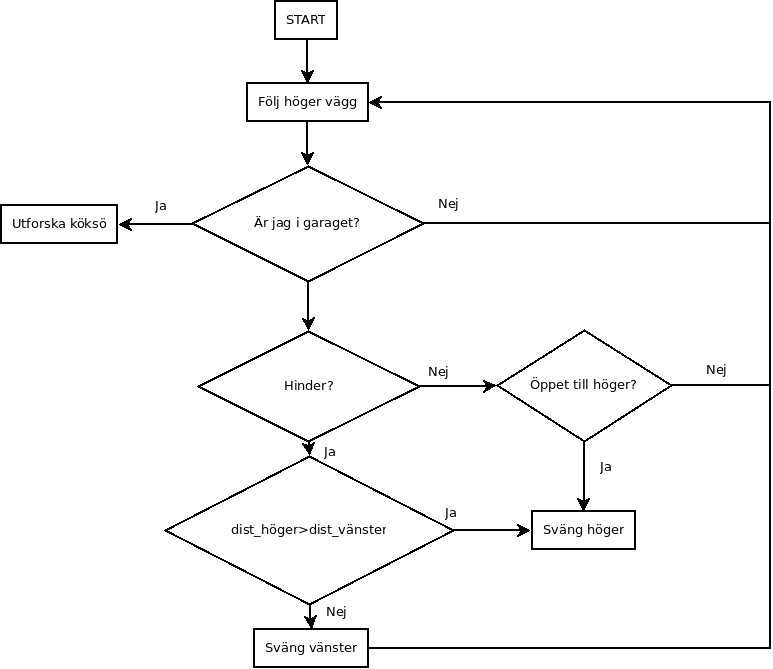
\includegraphics[width=0.8\textwidth]{autonomt_flowchart.png}}
	\caption{Flödesschema för det autonoma läget.  }
\end{figure}

%\begin{figure}[h!]
%\centering
%\begin{tikzpicture}[node distance=2cm,scale=0.6, every node/.style={scale=0.6}]
%
% Skiss:
% Är rummet klarskannat? -Ja-> vägleta till startplats -> klar
%   |        ʌ
%  Nej       |
%   |        ----------------------------------------------------
%   V                                                           |
%  Hitta lämplig rand till outforskat område -> vägleta dit -> skanna
%
% Styles
%\tikzstyle{startstop} = [rounded rectangle, minimum width=3cm, minimum height=1cm,text centered, draw=black, fill=red!30, align=center, inner sep=10pt]
%\tikzstyle{io} = [trapezium, trapezium left angle=70, trapezium right angle=110, minimum width=3cm, minimum height=1cm, text centered, draw=black, fill=blue!30, align=center, inner sep=10pt]
%\tikzstyle{process} = [rectangle, minimum width=3cm, minimum height=1cm, text centered, draw=black, fill=orange!30, align=center, inner sep=10pt]
%\tikzstyle{decision} = [diamond, minimum width=3cm, minimum height=1cm, text centered, draw=black, fill=green!30, align=center, inner sep=10pt, aspect=2]
%\tikzstyle{arrow} = [thin,->,>=stealth]
% Nodes
%\node (start) [startstop] {Start};
%\node (complete_map) [decision, below of=start, yshift=-40pt] {Room completely mapped?};
%\node (find_border) [process, left of=complete_map, xshift=-200pt] {Find appropriate border to unmapped area};
%\node (pathfind) [process, below of=find_border] {Pathfind there};
%\node (scan) [process, below of=pathfind] {Scan};
%\node (update_map) [process, right of=scan, xshift=200pt] {Update internal map};
%\node (pathfind_start) [process, right of=complete_map, xshift=150pt] {Pathfind to start};
%\node (done) [startstop, above of=pathfind_start, yshift=40pt] {Done};
% Arrows
%\draw [arrow] (start) -- (complete_map);
%\draw [arrow] (complete_map) -- node[anchor=south] {No} (find_border);
%\draw [arrow] (find_border) -- (pathfind);
%\draw [arrow] (pathfind) -- (scan);
%\draw [arrow] (scan) -- (update_map);
%\draw [arrow] (update_map) -- (complete_map);
%\draw [arrow] (complete_map) -- node[auto] {Yes} (pathfind_start);
%\draw [arrow] (pathfind_start) -- (done);
%\end{tikzpicture}
%\caption{Typiskt programflöde i det autonoma läget.}
%\label{fig:auto_flowchart}
%\end{figure}

\subsection{Gränssnitt} \label{ssec:brainInterface}
Kommunikations- och kontrollenheten använder sig av seriella bussar för datautbyte mellan sensorenhet och styrenhet. Mjukvara för dessa krävs på båda håll. Utbyte av data sker åt båda hållen; sensorenheten skickar data på kommando, och styrenheten skickar avläsningsdata.

Utöver detta finns Wi-Fi-kommunikation. Raspberry PI:ns inbyggda Wi-Fi-modul används. På båda sidor används sockets.

\newpage
\section{PC} \label{sec:system4}
Detta delsystem kommunicerar med Kommunikations- och kontrollenheten (se kapitel \ref{sec:system3}) för att ta emot diagnostisk data, den upptäckta kartan, samt ge instruktioner vid manuellt läge. Se figur \ref{fig:unitPC} för ett övergripande blockschema över PC-hårdvaran.

\begin{figure}[h!]
    \makebox[\textwidth][c]{
\includegraphics[width=0.6\textwidth]{PC.png}}
    \caption{Översikt över PC-modulen.}
    \label{fig:unitPC}
\end{figure}
\subsection{Hårdvara}
PC-mjukvaran ska vara körbar på en godtycklig PC med Python 3 och Wi-Fi-modul. Lämpligen med skärm, tangentbord, och datormus för kommunikation med användaren.

\subsubsection{Komponentbudget}
Här följer en lista på all hårdvara som detta delsystem kräver.

\begin{center}
\begin{HardwareList}
\hardware{PC}{PC med Wi-Fi-modul.}{1}
\end{HardwareList}
\end{center}

\clearpage

\subsection{Mjukvara}
PC-mjukvaran ansvarar för att kommunicera med roboten över Wi-Fi, låta användaren skicka kommandon till roboten, och visa diagnostik från roboten såväl som kartan. Se figur \ref{fig:gui_flowchart} för ett övergripande flödeschema för PC-mjukvaran. Koden är skriven i Python 3, och ska följa \cite{pep8}. Den består av två trådar där den ena hanterar GUIt och den andra hanterar kommunikation med roboten via en socket och med GUIt via köer.

\begin{figure}[h!]
\centering
\begin{tikzpicture}[node distance=2cm,scale=0.6, every node/.style={scale=0.6}]
% Styles
\tikzstyle{startstop} = [rounded rectangle, minimum width=3cm, minimum height=1cm,text centered, draw=black, fill=red!30, align=center, inner sep=10pt]
\tikzstyle{io} = [trapezium, trapezium left angle=70, trapezium right angle=110, minimum width=3cm, minimum height=1cm, text centered, draw=black, fill=blue!30, align=center, inner sep=10pt]
\tikzstyle{process} = [rectangle, minimum width=3cm, minimum height=1cm, text centered, draw=black, fill=orange!30, align=center, inner sep=10pt]
\tikzstyle{decision} = [diamond, minimum width=3cm, minimum height=1cm, text centered, draw=black, fill=green!30, align=center, inner sep=10pt, aspect=2]
\tikzstyle{arrow} = [thin,->,>=stealth]

% Nodes
\node (start) [startstop] {Start};
\node (wifi) [process, below of=start] {Establish Wi-Fi \\ connection};
\node (get_gui_event) [io, below of=wifi] {Get GUI event};
\node (command_issued) [decision, below of=get_gui_event, yshift=-0.8cm] {GUI command \\ issued?};
\node (should_transmit) [decision, below of=command_issued, yshift=-2cm] {Should \\ command be \\ transmitted?};
\node (perform) [process, right of=should_transmit, xshift=4cm] {Perform command};
\node (is_shutdown) [decision, right of=perform, xshift=3.5cm] {Command is \\ shutdown?};
\node (stop) [startstop, below of=is_shutdown, yshift=-1cm] {Stop};
\node (transmit) [process, below of=should_transmit, yshift=-1cm] {Transmit command};
\node (expecting_reply) [decision, below of=transmit, yshift=-1cm] {Query expecting \\ reply?};
\node (read_reply) [io, below of=expecting_reply, yshift=-1cm] {Read reply};
\node (should_update) [decision, below of=read_reply, yshift=-1cm] {Reply should \\ update GUI?};
\node (issue_event) [process, below of=should_update, yshift=-1cm] {Issue GUI event};

% Arrows
\draw [arrow] (start) -- (wifi);
\draw [arrow] (wifi) -- (get_gui_event);
\draw [arrow] (get_gui_event) -- (command_issued);
\draw [arrow] (command_issued) -- node[auto] {Yes} (should_transmit);
\draw [arrow] (should_transmit) -- node[auto] {No} (perform);
\draw [arrow] (perform) -- (is_shutdown);
\draw [arrow] (is_shutdown) -- node[auto] {Yes} (stop);
\draw [arrow] (is_shutdown) |- node[anchor=east, xshift=0.8cm, yshift=-5cm] {No} (get_gui_event);
\draw [arrow] (should_transmit) -- node[auto] {Yes} (transmit);
\draw [arrow] (transmit) -- (expecting_reply);
\draw [arrow] (expecting_reply) -- node[auto] {Yes} (read_reply);
\draw [arrow] (read_reply) -- (should_update);
\draw [arrow] (should_update) -- node[auto] {Yes} (issue_event);

% Common decision arrows
\coordinate[left of=get_gui_event, xshift=-3cm] (d1);
\coordinate[left of=issue_event, xshift=-85pt] (d2);
\draw [arrow] (d1) -- (get_gui_event);
\draw [-] (d1) to[below] node[auto] {} (d2);
\draw [-] (issue_event) to[left] node[auto] {} (d2);

\coordinate[left of=should_update, xshift=-85pt] (d3);
\draw [-] (should_update) to[left] node[auto] {No} (d3);

\coordinate[left of=expecting_reply, xshift=-85pt] (d4);
\draw [-] (expecting_reply) to[left] node[auto] {No} (d4);

\coordinate[left of=command_issued, xshift=-85pt] (d5);
\draw [-] (command_issued) to[left] node[auto] {No} (d5);
\end{tikzpicture}
\caption{Typiskt programflöde.}
\label{fig:gui_flowchart}
\end{figure}

% TODO: De andra sektionerna har inte lagt upp det så här med Input/Output-sektioner
%         Kan vara värt att diskutera med resten av gänget eller anpassa sig för ett mer uniformt dokument.

\subsubsection{Input}
PC-mjukvaran tar emot sensordata, styrdata och, kartdata från kommunikationsenheten via Wi-Fi. Den tar också emot instruktioner från användaren i form av knapptryck och tangentbordskommandon.

\clearpage

\subsubsection{Output}
Mjukvaran skickar styrkommandon samt uppmaning om att läsa av sensorerna till roboten i dess manuella läge. Den kan också skicka kommandon om att växla mellan autonomt och manuellt läge, som då går före den fysiska brytaren på roboten.

\subsubsection{GUI}
Informationen som tas emot från roboten presenteras i ett grafiskt gränssnitt. Via det grafiska gränssnittet kan användaren kunna välja kommandon som ska skickas till roboten, se diagnostisk information, växla mellan manuellt och autonomt läge, samt se den hitintills genererade kartan och robotens position i denna. Se figur \ref{fig:gui_mockup} för en mockup.

Det grafiska gränssnittet är byggt med grafikbiblioteket \cite{tkinter}.

\begin{figure}[h!]
    \makebox[\textwidth][c]{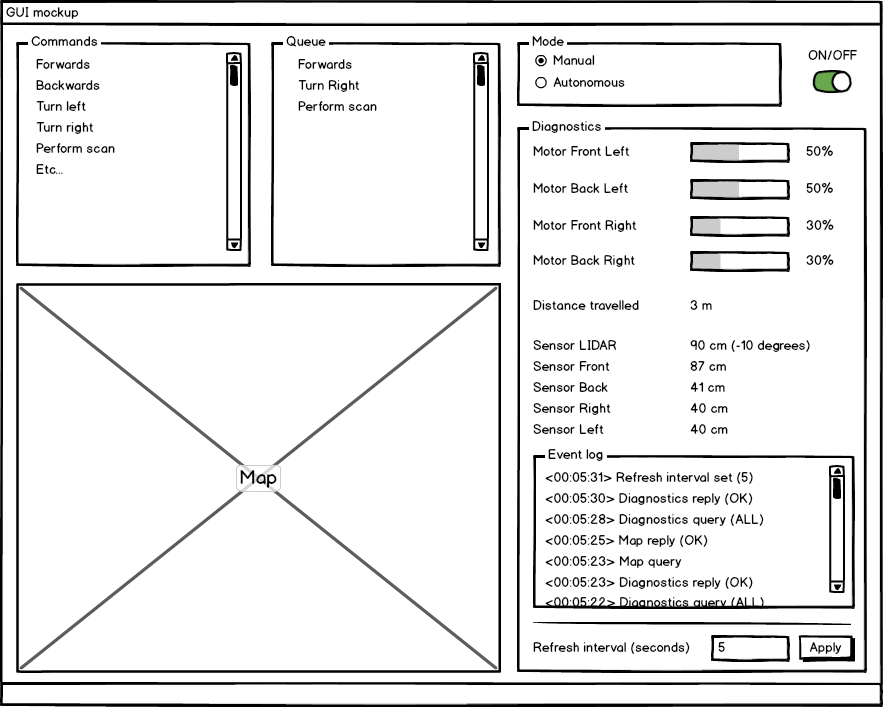
\includegraphics[width=0.8\textwidth]{gui_mockup.png}}
    \caption{Mockup av det grafiska gränssnittet.}
    \label{fig:gui_mockup}
\end{figure}

\subsection{Gränssnitt} \label{ssec:PCInterface}

PC:n kommunicerar med roboten över Wi-Fi. I mjukvarulagret används pythons inbyggda sockets.

\clearpage
\begin{appendices}

\section{Detaljerat blockschema}
\begin{figure}[h!]
    \makebox[\textwidth][c]{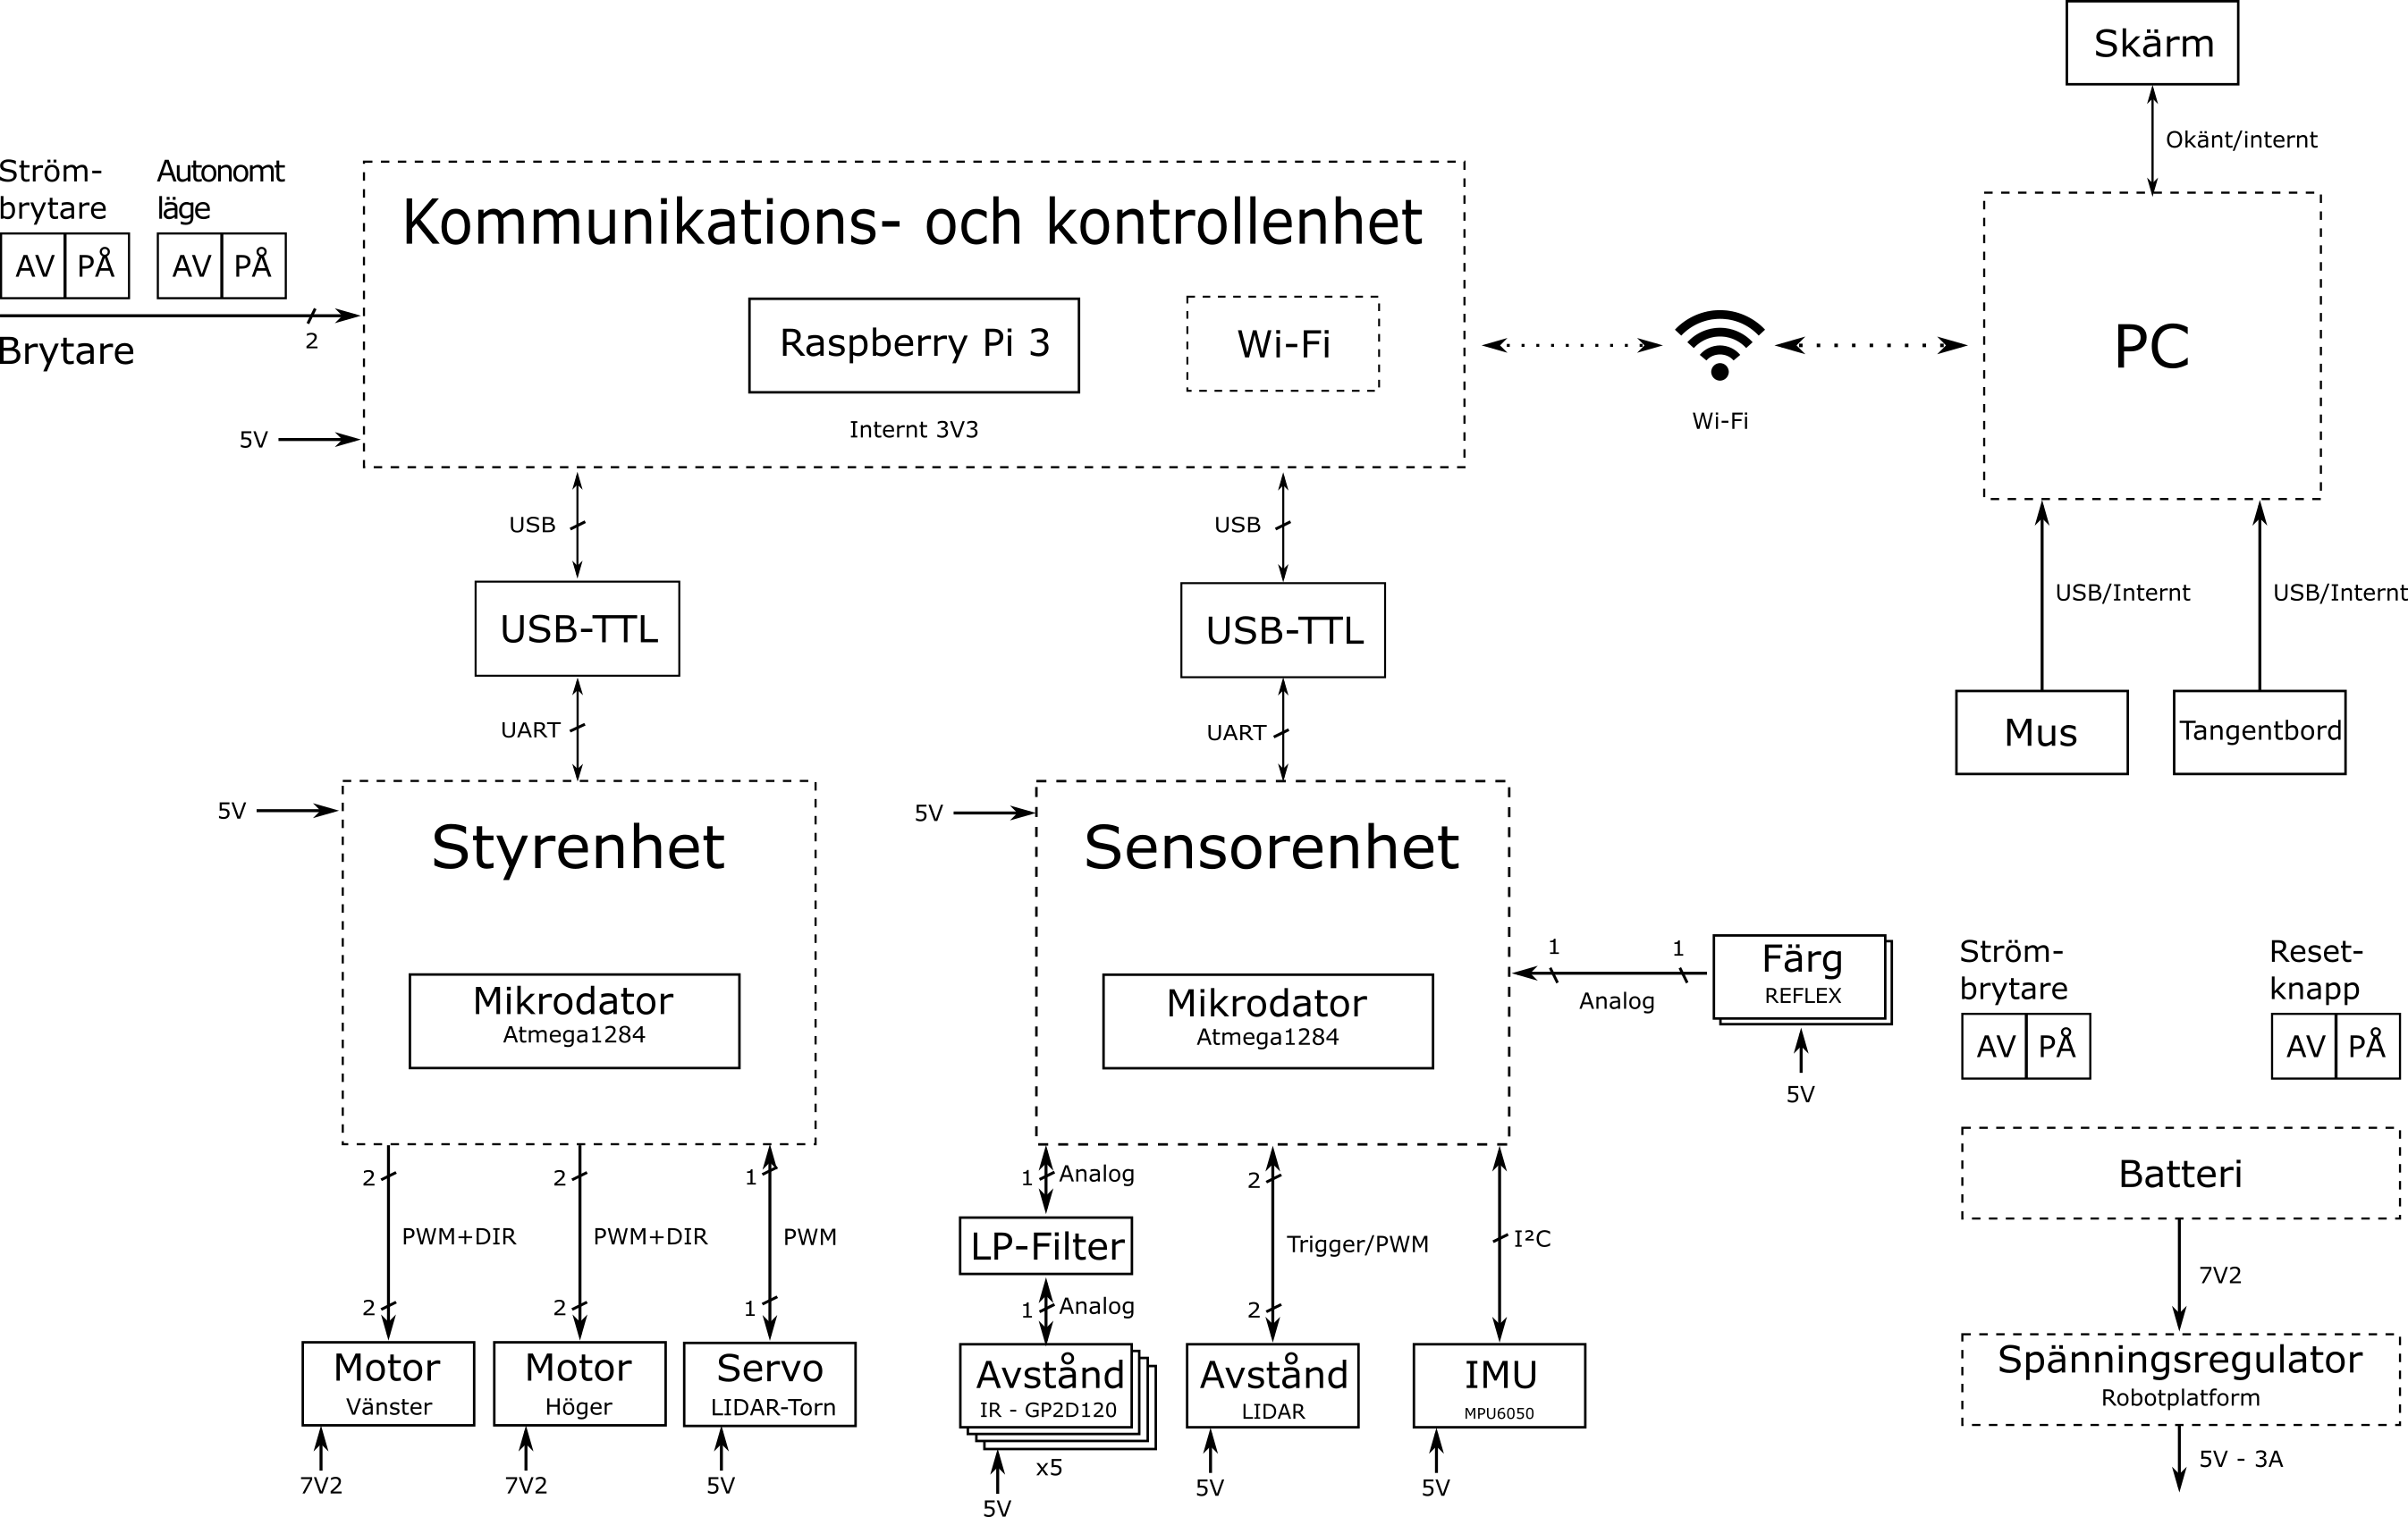
\includegraphics[width=1.1\textwidth]{modules_detail.png}}
    \caption{Detaljerat blockschema över systemet.}
    \label{fig:modulesDetailed}
\end{figure}

\includepdf[scale=0.8,pages=1,angle=180,pagecommand=\section{[Kopplingsschema] Styrenhet}\label{schematics:styrenhet}]{schematics/styrenhet/kicad.pdf}

\includepdf[scale=0.8,pages=1,angle=180,pagecommand=\section{[Kopplingsschema] Sensorenhet}\label{schematics:sensorenhet}]{schematics/sensorenhet/kicad.pdf}

\includepdf[scale=0.8,pages=1,angle=180,pagecommand=\section{[Kopplingsschema] Kontrollenhet}\label{schematics:brain}]{schematics/brain/kicad.pdf}

\clearpage
\section{C-standard} \label{sec:cstandard}
Som kodstandard för C används \cite{cstandard} med några smärre tillägg och ändringar:

\begin{itemize}
    \item Indenteringar sker med exakt fyra stycken mellanslag.
    \item Namn på funktioner, typedef, variabler, strukter, unioner, och enums ska vara i lower camel case.
    \item Namn på \#define's, enum-konstanter, och macrofunktioner ska vara i all-caps med ord separerade av underscore.
    \item Typedef:ade namn ska avslutas med "\_t".
    \item Globala namn ska \textit{ej} påbörjas med ett prefix som identifierar vilken modul de tillhör.
    \item Dokumentationskommentarer för funktioner och dylikt ska följa Doxygen-standard med JavaDoc-stil på inledande rad ("/**").
\end{itemize}

\clearpage
\section{Python-standard} \label{sec:pythonstandard}
Pythonkod följer \cite{pep8} med PyCharm-stil\footnote{\url{https://www.jetbrains.com/help/pycharm/2016.3/using-docstrings-to-specify-types.html}} på dokumentationskommentarer för funktioner och dylikt med vissa förändringar:

\begin{itemize}
    \item Indenteringar sker med exakt fyra stycken mellanslag.
    \item Alla dokumentationskommentarer för funktioner och dylikt ska inledas och avslutas med exakt tre dubbla, raka citationstecken (\texttt{"}) på ensam rad.
    \item För klassdokumentation används taggarna \texttt{:param} och \texttt{:attribute} för respektive konstruktorargument och publika attribut.
    \item Efter en parameter, attribut eller dylikt ska typen anges inom parentes.
    \item Taggar ska grupperas efter typ (såsom \texttt{:param}, \texttt{:return} och så vidare), och dessa grupper ska indenteras samt föregås av en rubrik som beskriver grupperingen.
\end{itemize}

\clearpage
\section{Robotplattform}
\label{app:placement}
\begin{figure}[h!]
    \makebox[\textwidth][c]{
\includegraphics[scale=0.6]{layout_topdown_vectorized.png}}
    \caption{Placering av hårdvara på robotchassit.}
    \label{fig:placement}
\end{figure}
\end{appendices}

\clearpage
\section{Programlistning}
\subsection{Huvudmoduler}
\subsubsection{Sensorenhet}
\dirtree{%
.1 /.
.2 dev.
.3 sensorenhet.
.4 Sensorenhet.
.5 Sensorenhet.
.6 Sensorenhet.c.
.6 Sensorenhet.h.
}

\begin{description}
\item[Redaktör] EN
\item[Författare] EN, SL, HH, JJ
\item[Datum] 2016-12-13
\item[Version] 1.0
\end{description}

\subsubsection{Styrenhet}
\dirtree{%
.1 /.
.2 dev.
.3 styrenhet.
.4 Styrenhet.
.5 Styrenhet.
.6 Styrenhet.c.
.6 Styrenhet.h.
}

\begin{description}
\item[Redaktör] DM
\item[Författare] DM, HH
\item[Datum] 2016-12-13
\item[Version] 1.0
\end{description}

\subsubsection{Kommunikations- och kontrollenhet}
\dirtree{%
.1 /.
.2 dev.
.3 kontrollenhet.
.4 main.py.
}

\begin{description}
\item[Redaktör] SL
\item[Författare] SL, FH, HH, DM, EN
\item[Datum] 2016-12-14
\item[Version] 1.0
\end{description}

\subsubsection{PC-mjukvara}
\dirtree{%
.1 /.
.2 dev.
.3 PC.
.4 main.py.
}

\begin{description}
\item[Redaktör] HH
\item[Författare] DM, HH, SL, EN
\item[Datum] 2016-12-14
\item[Version] 1.0
\end{description}

%\dirtree{%
%.1 /.
%.2 dev.
%.3 PC.
%.4 main.py.
%.3 kontrollenhet.
%.4 main.py.
%.3 styrenhet.
%.4 Styrenhet.
%.5 Styrenhet.
%.6 Styrenhet.c.
%.6 Styrenhet.h.
%.3 sensorenhet.
%.4 Sensorenhet.
%.5 Sensorenhet.
%.6 Sensorenhet.c.
%.6 Sensorenhet.h.
%}

\subsection{Dokumentationsstandard}
\subsubsection{C}
All funktionsdokumentation för den del av projektet som är skriven i C återfinns i header-filerna (\texttt{.h}).

\lstset{language=C,
                basicstyle=\ttfamily,
                keywordstyle=\color{blue}\ttfamily,
                stringstyle=\color{red!50!brown}\ttfamily,
                commentstyle=\color{green!50!black}\ttfamily,
                showstringspaces=false}
\begin{lstlisting}
#ifndef EXAMPLEMODULE_H_
#define EXAMPLEMODULE_H_

/**
 * @brief Example macro.
 */
#ifndef DEF_TEST
#define DEF_TEST 8000000UL
#endif

/**
  * @brief Example enum.
  */
typedef enum {VAL1, VAL2, VAL2, VAL4} enumExample_t;

/**
 * @brief Example function without return value.
 *
 * @param   param1 Description of param1.
 */
void startADConversion(type param1);

/**
 * @brief Example function with params and return value.
 *
 * @param   param1 Description of param1.
 * @param   param2 Description of param2.
 * @return  Description of return value.
 */
type msgTypeToSensor(type param1, type param2);

#endif /* EXAMPLEMODULE_H_ */

\end{lstlisting}

\clearpage
\subsubsection{Python}
\lstset{language=Python}
\begin{lstlisting}
"""
A short overview of this module, including usage examples
if necessary.

Examples:
        $ python3 main.py -f 'foo' -b 'bar'
"""

class ExampleClass:
    """
    Short description of this class including constructor
    arguments and public attributes.
    
    Args:
        param1  (type): Description of param1.

    Attributes:
        attr1   (type): Description of attr1.
        ATTR2   (type): Description of constant ATTR2.
    """

    def __init__(self, param1 : type):
        self.attr1 = param1
        self.ATTR2 = 10

    def function_with_return(self, param1: type):
        """
        Example function with return value.

        Args:
            :param1    (type): Description of param1.
        Returns:
            (type): Description of return value.
        """

    def function_without_return(self, param1: type, param2 : type):
        """
        Example function without return value.

        Args:
            :param1    (type): Description of param1.
            :param2    (type): Description of param2.
        """
\end{lstlisting}

\clearpage
\addcontentsline{toc}{section}{Referenser} %append references section at this location to TOC
\printbibliography
\end{document}
